\documentclass[titlepage]{article}
\usepackage{amsmath}
\usepackage{amssymb}
\usepackage{indentfirst}
\usepackage[margin=1in]{geometry}
\usepackage{longtable}
\usepackage{enumitem}
\usepackage{fancyvrb}
%\usepackage{graphicx}
\usepackage{pdfpages}
\usepackage{subcaption}
\usepackage{flafter}
\usepackage[section]{placeins}
\usepackage{float}
\hyphenation{wave-guide}
\renewcommand\_{\textunderscore\linebreak[1]}

\begin{document}

\begin{titlepage}

   \centering
   \vspace*{3cm}
   {\huge\bfseries OpenParEM2D User's Manual} \\
   \vskip1cm
   {\Large Version 2.1} \\
   \vskip1cm
   {\Large April 2025} \\
   \vskip1cm
   {\Large Brian Young} \\

   \vfill

   \includegraphics[width=0.5\textwidth]{figures/logo-crop}

   \vspace*{\fill}
   Copyright \copyright{} 2025 Brian Young. All Rights Reserved.
\end{titlepage}

%\newpage
\tableofcontents

\newpage
\section{Introduction}

OpenParEM2D is a full-wave electromagnetic simulator that solves the for the frequency-dependent complex propagation constant, characteristic impedance, and vector electric $(\overline{E})$ and magnetic $(\overline{H})$ fields of general 2D structures.  It is a free and open-source project released under the GPL3 license.

OpenParEM2D solves the full set of Maxwell's Equations (hence, full-wave) in the frequency domain on the x-y plane with the assumption that the only z-dependence of the fields are $e^{-\gamma z}$.  The solutions are mode of transmission lines and waveguides.  The fundamental mode and optionally higher-order modes are solved.

OpenParEM2D is a command-line tool that performs just the electromagnetic calculations.  To complete a project, other tools must be used to create a geometry, mesh the geometry, and plot results.  The complete set of tools and operations is called a flow, and any number of flows are possible.  The particular flow assembled for the development of OpenParEM2D is documented here.

This document covers how to use OpenParEM2D.  Details on the theory, methodology, and accuracy of OpenParEM2D are covered in a separate document "OpenParEM2D\_Theory\_Methodology\_Accuracy.pdf".

\section{Features}

OpenParEM2D features are listed in Table~\ref{table:features}, while anticipated future upgrades are listed in Table~\ref{table:upgrades}.

\begin{table}[ht]
\caption{OpenParEM2D List of Features}
\noindent \hrulefill
\begin{itemize}[nosep]
  \item Full-wave frequency-domain solution of Maxwell's Equations
  \item Arbitrary 2D geometries
  \item Arbitrary order finite elements
  \item Parallel processing using the Message Passing Interface (MPI)
  \item Adaptive mesh refinement
  \item PEC, PMC, and impedance (perturbational) boundary conditions
  \item Calculations
  \begin{itemize}
    \item complex propagation constant
    \item characteristic impedance
    \item dielectric loss
    \item conductor loss
    \item surface roughness loss
    \item field distributions
  \end{itemize}
  \item Dominant and higher-order modes
  \item Isotropic materials
\end{itemize}
\noindent \hrulefill
\label{table:features}
\end{table}

\begin{table}[ht]
\caption{OpenParEM2D List of Anticipated Future Upgrades}
\noindent \hrulefill
\begin{itemize}[nosep]
   \item Eliminate null-space solutions
   \item Finite element order ramping
   \item Non-perturbational impedance boundary
   \item Anisotropic materials
   \item One or more graphical user interfaces (GUI)
   \item Microsoft Windows\textsuperscript{\textregistered} port
\end{itemize}
\noindent \hrulefill
\label{table:upgrades}
\end{table}

\section{Characteristic Impedance}

From Maxwell's equations, the solution setup of a 2D cross-section of a transmission line or waveguide is an eigenvalue problem that on solving provides the complex propagation constant and electric field $\overline{E}$.  The magnetic field $\overline{H}$ can be solved as a post-processing operation.  Characteristic impedance is not a fundamental quantity when solving Maxwell's equations. Instead, it is calculated as a post-processing step on $\overline{E}$ and d $\overline{H}$ using any definition that meets the needs of the engineering design problem.  The user must set up the calculation for the characteristic impedance through the definition of integration paths for voltages and currents and the selection of the definition of the characteristic impedance to use.

The specific calculation chosen for the characteristic impedance should be the one that is most useful in an engineering sense.  The characteristic impedance is used to design for impedance matching to minimize reflections and for filter design, where reflections are controlled to produce a specific frequency response.  So the best calculation to use is the one that produces the closest match between simulation and measurement.  The best definition to use for one class of problems is not necessarily the best definition for another class of problems.

\subsection{Definitions}

Fundamentally, all solutions to the 2D problem are the modes of the structure, where each \textit{mode} represents a unique solution to the eigenvalue problem with a unique field structure and complex propagation constant.  For many users, only one mode is needed, which is referred to as the \textit{dominant mode}.  The electromagnetic modes are analogous to a string fixed on each end that is plucked, where there is a fundamental vibration plus harmonics.  The fundamental tone is the dominant mode, and the harmonics represent the higher-order modes.

Each mode has its own unique field structure, so each also has its own unique characteristic impedance requiring a unique setup.  In OpenParEM2D setups, configurations that apply directly to one given mode are called \textit{modal} setups.  In practice, this means that voltage and/or current integration paths specific to each mode must be defined.

For multiconductor transmission lines as seen in printed circuit boards and semiconductor packages, the modal setups are not known except for the special case of differential pairs (i.e. a multiconductor transmission line with just two symmetric signal conductors plus a ground plane).  For multiconductor transmission lines, OpenParEM2D supports the definition of non-modal integration paths for the voltages and currents then applies an algorithm to compute the modal voltages and currents from the non-modal integration paths.  These non-modal integration paths are called \textit{line} setups.

Of the infinite number of possible definitions for the calculation of characteristic impedance, OpenParEM2D supports the three primary definitions, and it is at the user's discretion as to which definition to use for any given application.  The three implemented definitions for the characteristic impedance, $Z_\circ$, are the power-voltage (PV) definition given by
\begin{equation}
Z_\circ=\frac{1}{2}\frac{VV^*}{P_z^*},
\end{equation}
the power-current (PI) definition given by
\begin{equation}
Z_\circ=2\frac{P_z}{II^*},
\end{equation}
and finally, the voltage-current (VI) definition as
\begin{equation}
Z_\circ=\frac{V}{I},
\end{equation}
where $V$ and $I$ are the voltage and current, respectively, and $P_z$ is the power propagating in the $z$-direction.  The $P_z$ term is always calculated for all modes, so the user does not need to set up anything for it.  However, the voltage and current need further consideration.

\subsection{Single-Mode Setups}

In practice, most  applications only use the dominant mode, for which the setups for the voltage and current are well known.  For single-mode setups, integration paths for the voltage, the current, or both must be provided.  If just the voltage path is provided, then only the PV definition can be calculated.  Similarly, if just the current path is provided, then only the PI definition is available.  If both are provided, then both definitions are calculated, and finally, if neither is provided, then no characteristic impedance is calculated.
In the single-mode case, modal and line integration path setups are identical, use the same calculation, and produce the same result for the characteristic impedance. 

\subsection{Multi-Mode Setups}

When more than one mode is requested, voltage and current integration paths must be defined by the user for the dominant and higher-order modes, and the definitions vary per mode.  If definitions are not provided for a mode, then the characteristic impedance for that mode is not calculated.

The voltage and current paths must be provided by the user customized for each mode using modal setups.  For the special case of multiconductor transmission lines, the user has the option of providing line setups instead of modal setups.  With a line setup, non-modal voltages and currents are extracted from the 2D fields and combined to calculate the modal voltages and currents.  This relieves the user of the need to define the modal integration paths, which are only known for differential pairs.  Either setup ultimately calculates the modal voltages and currents and currents leading to modal characteristic impedances.

Consider the case of the differential pair shown in Fig.~\ref{fig:multimode}, which is marked with two current paths, \texttt{\_P1} and \texttt{\_P2}, and two voltage paths, \texttt{\_P3} and \texttt{\_P4}.
\begin{figure}
  \centering
  \includegraphics[width=0.5\textwidth]{./figures/multimode2}
  \caption{A differential pair marked with voltage and current integration paths.}
  \label{fig:multimode}
\end{figure}
For \textit{modal} setups, one current path and/or one voltage path must be defined per mode.  For the even mode (common mode), the currents on the conductors are equal, and the current is calculated over the total path of \texttt{\_P1$+$\_P2}.  The voltages on the two conductors are equal, so the voltage is calculated on \texttt{\_P3} or \texttt{\_P4} or as 1/2 of the voltage calculated on the path \texttt{\_P3$+$\_P4}.  For the odd mode (differential mode), the currents are equal and opposite, and the current is calculated as the current on \texttt{\_P1} or \texttt{\_P2} or as 1/2 the current calculated over the path \texttt{\_P1$-$\_P2}.  The voltage is calculated as the total voltage the path \texttt{\_P3$-$\_P4}.  For asymmetric differential pairs or multiconductor transmission lines with more than 2 conductors, the splits of the currents and voltages on the integration paths are not simple, so they are challenging to set up.

For line setups, combinations of the paths in Fig.~\ref{fig:multimode} are not attempted.  Instead, the voltages and currents are calculated for the individual paths as drawn.  Since these are defined on a per-line basis instead of a per-mode basis, this setup is called the \textit{line} setup.  By themselves, the line voltages and currents are meaningless, but once combined, they yield the modal voltages and currents.  For the differential pair in Fig.~\ref{fig:multimode}, two sets of voltages and currents are calculated using the line integration paths: one for the even mode and one for the odd mode.  For the even mode, the computed line currents are $I_1^e$ and $I_2^e$, and the line voltages are $V_3^e$ and $V_4^e$.  Similarly for the odd mode, the computed line values are $I_1^o$, $I_2^o$, $V_3^o$, and $V_4^o$.  The even mode current is then $I^e=I_1^e+I_2^e$, and the even mode voltage is $V^e=1/2(V_3^e+V_4^e)$.  For the odd mode, $I^o=1/2(I_1^o-I_2^o)$ and $V^o=V_3^o-V_4^o$.

For multiconductor transmission lines with line setups, OpenParEM2D applies a general algorithm to combine line currents and voltages to obtain modal currents and voltages.  In the symmetric case of a differential pair, the algorithm produces the result just described.  OpenParEM2D cannot know whether a drawing is a multiconductor transmission line, so if a line setup is applied by the user, then the algorithm is applied whether or not it is appropriate.  In general, modal setups should be used except for multiconductor transmission lines.

In summary, with a modal setup, the user provides integration paths for voltages and currents customized per mode to obtain the correct modal voltages and currents.  For a multiconductor transmission line, the user has the option of providing a line setup with voltage and current paths defined per line, then OpenParEM2D applies an algorithm to combine the line voltages and currents to obtain modal voltages and currents.  When properly set up, the two approached produce the same characteristic impedance for each mode.

\section{Files}
\label{sec:files}

OpenParEM2D is a command-line tool that takes one and only one input, and that is a text project control file.  To run serially on a single core or processor, the command is
\begin{Verbatim}[fontsize=\small]
   $ OpenParEM2D project_name.proj
\end{Verbatim}
and in parallel it is
\begin{Verbatim}[fontsize=\small]
   $ mpirun -q --oversubscribe -np N OpenParEM2D project_name.proj
\end{Verbatim}
where \texttt{project\_name.proj} is the project control file.  See Sec.~\ref{sec:solution} for details on the switch settings \texttt{-q}, \texttt{-oversubscribe}, and \texttt{-np}. To view a very short help message and the version number, execute
\begin{Verbatim}[fontsize=\small]
   $ OpenParEM2D -h
\end{Verbatim}

All inputs are captured in the project control file including names of files that must be included. So setting up a project involves creating/editing a project control file and ensuring that the additionally required files are specified and available.

The required include files in a project control file define materials, mesh, and port definitions. Each of the required files are covered in detail in the following sections.

\subsection{Project Control File}

All aspects of the execution of OpenParEM2D are controlled by the project control file.  There are no other inputs or command line options.  The file consists of a list of keyword/value pairs that are documented in Appendix~\ref{sec:control_file_spec}.  A simple but working control file is shown below.

\begin{Verbatim}[fontsize=\small]
   #OpenParEM2Dproject 1.0
   project.save.fields               false
   mesh.file                         coax.msh
   mesh.order                        2
   mode.definition.file              coax_modes.txt
   materials.global.path             ../
   materials.global.name             global_materials.txt
   refinement.frequency              high
   refinement.variable               |Zo|
   refinement.iteration.min          3
   refinement.iteration.max          50
   refinement.required.passes        1
   refinement.tolerance              1e-5
   frequency.plan.log                1e7,10e9,1
   solution.modes                    1
   solution.impedance.definition     PV
   solution.impedance.calculation    modal
\end{Verbatim}

\noindent In this example setup, the mesh file "coax.msh" is generated using gmsh \cite{gmsh}\cite{gmshweb}, the coax\_modes.txt file is generated using the script "OpenParEM2D\_save.py" in FreeCAD \cite{FreeCAD}, and the materials file "global\_materials.txt" is a hand-generated library file used across many projects.
Keyword/value pairs can be added to the control file to do things like outputting files to enable plotting with ParaView \cite{ParaView} [project.save.fields true] or calculate field values at specific (x,y) points [field.point 0,0.0008].

The names of the files generated by OpenParEM2D are based on the name of the project control file with the extension removed.  So a control file called "my\_project.proj" results in new files and directories being created called "my\_project\_results.csv", "ParaView\_my\_project", "temp\_my\_project", etc.  The files are uniquely identified by the project name, so more than one project can exist in a single directory without file name conflicts.


The text-based control file has several advantages, with a few techniques listed here.
\begin{itemize}[nosep]
  \item Project control files tend to be similar across projects, so common practice is to copy a control file from an old project to a new one and then edit as necessary.
  \item A project can have multiple control files to explore simulation strategies.  A simple comparison of project control files [e.g. Linux diff or sdiff] shows the differences in setup.
  \item Directory trees can be easily searched to find projects using or not using certain simulation features using the helper tool "proj\_search".  As completed projects accumulate, this feature becomes more useful.
  \item Comments can be used to add notes and keep track of changes or variations.  In a GUI, the only option for the user is to check/uncheck a box or to change a number.  With a text-based setup file, the change can not only be made, but the \textit{reason} for the change can be given or the \textit{history} of the setting can be maintained.  This is a surprisingly capable feature that should be liberally used.
\end{itemize}

The frequencies to solve and the frequencies and order for adaptive mesh refinement are defined in a \textit{frequency plan}.  OpenParEM2D sets up frequency plans identically to OpenParEM3D, and the definition and use of frequency plans are covered in "OpenParEM3D\_User\_Manual.pdf".

\subsection{Materials Files}

Materials use the same materials files as described in "OpenParEM3D\_User\_Manual.pdf".

\subsection{Mesh File}

The supported mesh file formats are gmsh v.2.2 and the native format of MFEM \cite{MFEM}\cite{MFEMweb}.  When setting up a project, the general procedure is to use a CAD program that can output geometry data readable by gmsh, then use gmsh to mesh the structure and output a gmsh v2.2 mesh file.  The mesh file is then specified in the project control file using the \texttt{mesh.file} keyword.  To get the v.2.2 mesh output from gmsh, the format must be specified on the command line when starting gmsh as follows
\begin{Verbatim}[fontsize=\small]
   $ gmsh -format msh22 &
\end{Verbatim}
\noindent One free and open-source CAD program that is supported by gmsh is FreeCAD.  FreeCAD outputs a *.brep file that can be imported by gmsh.

\subsection{Mode Definition File}
\label{sec:mode_definition_file}

Modes and boundaries are specified in a text file following the specification in Appendix~\ref{sec:mode_file_spec}.  The project control file specifies the mode definition file using the \texttt{mode.definition.file} keyword. Due to complexity, the mode definition file is very difficult to write by hand, so scripted generation is generally required.  When using FreeCAD, the Python script "OpenParEM2D\_save.py" can be used to generate the mode definition file.


\section{Example Projects}

An automated regression suite is in place as part of the release methodology. The projects in the suite are listed in Appendix~\ref{sec:regression_suite}.  The suite also represents a large number of worked examples that are ready to run with known answers.  For example, for the regression project \texttt{WR90\_rectangular\_waveguide/WR90/WR90\_order\_4\_refinement/WR90.proj}, the project can be run at the command line by executing
\begin{Verbatim}[fontsize=\small]
   $ process.sh WR90.proj 5
\end{Verbatim}
where depending on the computer, a number smaller or larger than 5 could be appropriate for the number of cores to use.  At successful completion, the file "WR90\_test\_results.log" can be viewed for summary results and "straight\_test\_test\_results.csv" for a detailed pass/fail report.  Results for the complex propagation constant, characteristic impedance, voltage, current, and power are available in "WR90\_test\_results.csv".  Computed values for the fields are available in "WR90\_test\_fields.csv".  To view the fields, set \verb+project.save.fields true+ before running the project, then run ParaView to setup and view fields.

The regression suite cases are set up for more accuracy than needed for engineering work to enable tight pass/fail criteria to be set.  In many situations, looser settings are appropriate.

The accuracy demonstrations listed in Sec.~\ref{sec:studies} provide additional worked examples.  These are set up for maximum accuracy and accept relatively slow run times.

\section{Flow}

The process of setting up and running a project from scratch involves several steps: draw the geometry via CAD or script, create a mesh, define ports and set boundary conditions [if needed], create a local materials file if the needed materials do not exist in the global library file, and finally run OpenParEM2D.  Except for the OpenParEM2D step, any number of tools and techniques can be used to generate the needed files.  One methodology is described here.

\subsection{Geometry Definition Using FreeCAD}
\label{sec:freecad}

FreeCAD is an effective tool for building complex 2D geometries for simulations.  It does have a significant learning curve, but tips are provided to help with that.  Start FreeCAD with
\begin{Verbatim}[fontsize=\small]
   $ freecad &
\end{Verbatim}
\noindent then start a new project with \texttt{File}$\rightarrow$\texttt{New}.
At first use, set some preferences starting with \newline \texttt{View}$\rightarrow$\texttt{Workbench}$\rightarrow$\texttt{Draft} then \texttt{Edit}$\rightarrow$\texttt{Preferences ...}.
Click on the \texttt{General} icon then on the \texttt{General} tab and set the \texttt{Unit system:} to \texttt{Standard (mm, kg, s, degree)} and \texttt{Number of digits:} to 3.
Next click on the \texttt{Draft} icon and then the \texttt{General settings} tab and set the \texttt{Internal precision level} to 10. Finally, click on the \texttt{Draft} icon and then the \texttt{Grid and snapping} and set the \texttt{Grid spacing} to 1 $\mu$m to enable drawing at $\mu$m scale as discussed next on the unit system in FreeCAD.

An important note about the unit system is that FreeCAD has internal scaling that does not seem to adhere to the length units of mm.  Drawing in mm will generally lead to the mesh being output in m.  This seems strange for its use here, but it must work in other scenarios.  Or, perhaps a setting has been missed.  Generally, drawings must be made in $\mu$m to get mm scaling in the final mesh, or the drawing can be done in mm then scaled by 0.001 in the x-, y-, and z- directions.

To continue with drawing, FreeCAD should be in the Draft Workbench by selecting \newline\texttt{View}$\rightarrow$\texttt{Workbench}$\rightarrow$\texttt{Draft}.  The next step is critical to avoid a very messy drawing experience.  On the toolbar, click the \texttt{Auto} button then click \texttt{Top (XY)} to set the drawing plane.  The drawing plane is where 2D primitives such as lines and rectangles are drawn.

To build a 2D model, primitives such as lines and rectangles are drawn on the drawing plane.  It is important to use the snap functionality to ensure that objects are aligned.  Once drawn, editing of an object is often easier by editing the text parameters rather that using mouse operations.

In addition to a typical copy operation, FreeCAD also has a clone operation.  The clone operation is very powerful because edits to the parent object cascades to the child cloned objects.  Use of clones does take some planning to ensure that changes to the parent are reflected in the clones in ways that make sense for the 2D model.

When the 2D model is complete, all of the components must be merged using the "boolean fragments" operation in the Part Workbench with \texttt{Part}$\rightarrow$\texttt{Split}$\rightarrow$\texttt{Boolean fragments}.  The resulting object can be exported using \texttt{File}$\rightarrow$\texttt{Export ...} to save with the BREP file format, which can be imported by gmsh for material assignment and meshing. 

If the 2D model is built in mm, then the boolean fragment object can be cloned, and the clone can be scaled in 3 dimensions by 0.001.  The scaled clone can then be exported as a BREP file.  A scaled clone loses the connection to the parent object, so a change to the parent requires the scaled clone to be deleted and re-created with a new clone.

FreeCAD has vastly more capability than that described here, and there are very likely alternative or better ways to get things done than those described in these tips.  Given its expansive capabilities and Python scripting support, it is highly likely that scripting could greatly simplify the process of building a 2D model for OpenParEM2D.

\subsection{Mode and Boundary Annotation Using FreeCAD}

The required mode definition file can be built by hand, but that is not generally practical.  The FreeCAD Python script "OpenParEM2D\_save.py" can be used to generate the needed mode definition file once the 2D model has been annotated with the needed mode and boundary information.  The annotations are added as physical objects, such as lines, rectangles, and polylines, along with text objects providing instructions to "OpenParEM2D\_save.py". 

\subsubsection{Paths (\_P)}
\label{sec:paths}

Paths are physical drawing elements used as voltage and current integration paths.  Lines, rectangles, and polylines can be added to the drawing then marked as paths by editing the \texttt{Label} property in the property box to
\begin{Verbatim}[fontsize=\small]
  _Ppathname
\end{Verbatim}
\noindent where \texttt{pathname} can be any text with alphanumeric characters.  The paths are referenced by other annotations only by \texttt{pathname}, so the \texttt{\_P} part is dropped.

\subsubsection{Integration Paths (\_M, and \_L)}
\label{sec:integration_paths}

Integration paths for voltages and currents are set up using previously defined paths plus additional information indicating voltage or current plus [optionally] scale. An integration path is added to the drawing by placing a text object with any text, which is ignored.  A simple period works well.  The integration path information is entered by editing the \texttt{Label} property of the added text object located in the property box to
\begin{Verbatim}[fontsize=\small]
  _Mmodenumber(voltage|current[,scale]){[+|-]pathname1,+pathname2,-pathname3,...}
\end{Verbatim}
\noindent or
\begin{Verbatim}[fontsize=\small]
  _Lmodenumber(voltage|current[,scale]){[+|-]pathname1,+pathname2,-pathname3,...},
\end{Verbatim}
\noindent where \texttt{modenumber} is an integer, \texttt{scale} is a scale factor for the computed results [default=1], and the pathnames define the path.  The pathnames string together, where $+$ and $-$ signs allow reversing direction, if needed.  The two forms (\textit{\_M} or \textit{\_L}) are identical except for the prefix, which determines whether modal or line calculations are used to obtain the voltages and currents.  For each modenumber, two entries are allowed: one for voltage and one for current.

OpenParEM2D solves for the dominant and higher-order modes, and the modes are sorted so that they are ordered from highest to lowest effective dielectric constant.  The voltage and/or current integration paths defined for modenumber=1 are applied to the mode with the highest effective dielectric constant. The mode with the next highest effective dielectric constant is used with the integration paths defined with modenumber=2, and so on.  It is required that modenumber start with 1 and increase sequentially.

\subsubsection{Boundaries (\_B)}

Boundaries conditions are defined by placing a text object with any text, which is ignored, with the \texttt{Label} property in the property box edited to
\begin{Verbatim}[fontsize=\small]
  _Bboundaryname(SI|PEC|PMC[,material]){[+|-]path,-path,+path,...}
\end{Verbatim}
\noindent where \texttt{boundaryname} can be any alphanumeric text, the boundary type is selected as one of \texttt{SI} for surface impedance, \texttt{PEC} for perfect electric conductor, and \texttt{PMC} for perfect magnetic conductor.  Selecting \texttt{SI} requires the conductor material to be specified in the second argument [e.g. copper].

A PEC boundary forces the electric field tangential to the boundary to be exactly zero.  This is the default boundary condition for any edge facing outside to an area that does not have a defined dielectric.
 The PEC boundary is useful for enforcing symmetry to reduce the size of the computational space for problems with anti-symmetric electric fields and symmetric magnetic fields.

A PMC boundary forces the magnetic field tangential to the boundary to be exactly zero.  The PMC boundary is useful for enforcing symmetry to reduce the size of the computational space for problems with symmetric electric fields and anti-symmetric magnetic fields.

An SI boundary assumes that the conductor is thick compared to the skin depth at the simulation frequency.  No penetration through the boundary is modeled.

\subsection{Meshing Using gmsh}
\label{sec:gmsh}

For meshing, gmsh is an effective tool that has a relatively straightforward interface.  The library used by OpenParEM2D only supports the version 2.2 mesh format from gmsh, so it must be started calling for this format as
\begin{Verbatim}[fontsize=\small]
   $ gmsh -format msh22 &
\end{Verbatim}
\noindent Open the BREP file exported from FreeCAD with \texttt{File}$\rightarrow$\texttt{Open ...} then select a file with the \texttt{.brep} extension.

Before meshing, materials must be assigned to the surfaces in the imported model.  In the cascading options, select $\boxplus$\texttt{Geometry}$\rightarrow$$\boxplus$\texttt{Physical groups}$\rightarrow$$\boxplus$\texttt{Add}$\rightarrow$\texttt{Surface}.  A popup menu appears along with crossing dotted lines on the model indicating the surfaces.  Add text to the popup for the material for a specific surface, then click a crossing line (or more, if all have the same material) for that surface, then enter \texttt{e} on the keyboard to complete the entry.  A popup will appear to create a file with a \texttt{.geo} extension, and accept that.  Continue until all surfaces have materials assigned, then enter \texttt{q} to quit.  Note that sometimes entry by the mouse is disabled, indicated by a red box in the lower left-hand corner, so if the mouse becomes disabled, click that red box.

With the materials defined, in the cascading options select $\boxplus$\texttt{Mesh}$\rightarrow$\texttt{2D} to generate a mesh.  If the mesh is acceptable, then in the cascading options select \texttt{Save} to save the mesh with an automatic \texttt{.msh} extension.  Gmsh can be closed without needing to save any information because the \texttt{.geo} file is automatically saved.
On re-opening a project, load the \texttt{.geo} to pick up the surface assignments.  Meshing can then immediately proceed.

At the GUI level, meshing behavior can be modified by opening a control panel with \texttt{Tools}$\rightarrow$\texttt{Options}.  An options window will appear, then select \texttt{Mesh}$\rightarrow$\texttt{General}.  The primary controls are the 2D algorithm and the element size factor.  At this point, it is up to experimentation to see what works best for the geometry at hand.  After a mesh is generated, a change in settings is made by selecting in the cascading options $\boxplus$\texttt{Geometry}$\rightarrow$\texttt{Reload script} to clear the existing mesh, then make any changes to the meshing options and select $\boxplus$\texttt{Mesh}$\rightarrow$\texttt{2D} to generate a new mesh.

Generally, a sparse mesh is desirable for speed, but sparser meshes have lower quality, which impacts the ultimate speed and accuracy of the electromagnetic solution.  The mesh quality can be viewed by selecting \texttt{Tools}$\rightarrow$\texttt{Statistics}$\rightarrow$\texttt{Update}.  Several metrics are supplied, but the idea is to get these as close to 1 as possible, but generally, they will be far less than 1. 

Once a mesh is complete, select  \texttt{Files}$\rightarrow$\texttt{Save Model Options} to save the settings to a file with an automatic \texttt{.opt} extension.  The \texttt{.opt} is always applied so that new mesh generation can start where the last one left off.  To start over from scratch, delete the \texttt{*.opt} file before starting gmsh.

Beyond the simple use described here, gmsh has a vast array of features and options plus scripting capabilities. With the simple tips above, meshing can get started while additional capabilities are explored over time.

\subsection{Solution With OpenParEM2D}
\label{sec:solution}

Once the mode definition file from FreeCAD and the mesh file from gmsh have been generated, the project setup file can be completed with links to these and to a materials file.  With all of the files ready, a project file with the name \texttt{my\_project.proj} can be executed by 
\begin{Verbatim}[fontsize=\small]
   $ mpirun -q --oversubscribe -np N OpenParEM2D project_name.proj
\end{Verbatim}
where \verb+N+ is the number of cores to use for the calculation.  The switch \verb+-q+ is optional and eliminates extra messaging from the MPI system.  The switch \verb+--oversubscribe+ is required when \verb+N+ is greater than half the number of available cores, but otherwise, it is optional.  \verb+N+ should generally not exceed the number of available physical cores, and in most cases, best run times occur when \verb+N+ is less than the number of available cores.  Experimentation is required to find the value of \verb+N+ that results in the lowest run times for a specific computer.

For very small problems, setting \verb+N+ too large can cause OpenParEM2D to hang at the function call within the MFEM library that sets up the finite element problem.  The problem is that there is not enough data to spread among the number of requested processors.  There is not a way for OpenParEM2D to check and report when \verb+N+ is too large.  If OpenParEM2D hangs at the step \texttt{building finite element spaces ...}, then the remedy is to kill the job and re-start with a smaller \verb+N+.

It is likely on initial attempts to run a new setup with OpenParEM2D that errors will be reported and the simulation stopped.  The design of OpenParEM2D is to make no assumptions or corrections to input decks, so every error is reported even if it could be possible for OpenParEM2D to fix or adjust the setup.  Correct the errors and try again.

OpenParEM2D uses a lock file to prevent data collisions from accidentally running the same project file more than once at a time.  The project lock file has the form \texttt{.project\_name.lock}.  Should a running job exit unexpectedly, the lock file can be deleted as 
\begin{Verbatim}[fontsize=\small]
   $ rm .project_name.lock
\end{Verbatim}
\noindent so that the job can be restarted.  Since the name starts with a period, it is a hidden file, so to see the lock file in a directory requires
\begin{Verbatim}[fontsize=\small]
   $ ls -a
\end{Verbatim}

The goal is that OpenParEM2D always detects problems and exits gracefully with an error message with the lock file removed.  Any other exit style is an issue that needs to be fixed with improved error checking, with one exception.  For a large project that runs out of memory, OpenParEM2D will exit with cryptic messages from the MPI system without mentioning the memory issue and without removing the lock file.

When a job is running, progress is shown by extensive data sent to the terminal.  This output should be redirected to a file if the simulation progress is to be logged.

\subsection{Viewing Fields}

To view the computed electromagnetic fields, OpenParEM2D outputs files for viewing with ParaView after every iteration and every frequency.  To enable this output, set
\begin{Verbatim}[fontsize=\small]
  project.save.fields true
\end{Verbatim}
\noindent in the project setup file.  After loading the result in ParaView, a very useful predefined set of plots can be generated by running the macro "field\_plot" from the \texttt{Macros} menu item.

Since the files are produced while OpenParEM2D is executing, ParaView can be used to view intermediate results.  The one constraint is that ParaView will report errors if OpenParEM2D updates the files while ParaView is still reading them.  If that happens, just try again.

The default behavior for ParaView is to enable the user to make several changes then click \texttt{Apply} to review the recomputed output.  This is good behavior for very large datasets but inconvenient for small ones.  A preference can be set to automatically implement changes immediately after every update.  This setting can be found at \texttt{Edit}$\rightarrow$\texttt{Settings ...}$\rightarrow$\texttt{General}$\rightarrow$\texttt{Auto Apply}.

After a ParaView file is opened, if the macro "field\_plot" is not run, then nothing is shown.  To show a result, scan down to the \texttt{Coloring} section where there is a dropdown box labeled \texttt{Solid Color}.  Change this setting to one of the field options.  For vectors, the displayed field can be further refined by changing from plotting \texttt{Magnitude} to one of the field components.


Beyond the simple use described here and the tutorials, ParaView has a vast array of filters and customizations forming a very powerful visualization capability. With the simple tips above, visualization can get started while additional techniques are explored over time.

\section{Results File}

Computed results are saved to a csv file called "project\_name\_results.csv".  A commented header line shows the content of each column.  The only outputs from OpenParEM2D are this file, the ParaView output, and the data printed to the terminal during execution.

\section{Tutorials}

\subsection{Rectangular Waveguide}
WR90 rectangular is constructed, annotated, meshed, and solved.  WR90 rectangular waveguide is 22.86 mm wide and 10.16 mm tall and has a recommended frequency range from 6.557 GHz to 13.114 GHz.

\subsubsection{Drawing and Mode Annotation}

\begin{itemize}
\item Create a directory for the project
\begin{Verbatim}[fontsize=\small]
$ mkdir rectangular_waveguide
$ cd rectangular_waveguide
\end{Verbatim}
\item Start FreeCAD, open a new drawing, set preferences [if needed], set the drawing workspace to \texttt{Draft}, and set the drawing plane to \texttt{Top} as outlined in Sec.~\ref{sec:freecad}.
\item Click \texttt{Drafting}$\rightarrow$\texttt{Rectangle} or click on the rectangle icon on the toolbar and draw a rectangle of any size by clicking to start then clicking to end.
\item Select the rectangle either on the drawing space or in the \texttt{Combo View} window.
\item In the \texttt{Property} window, for property \texttt{Height} change the value to 10.16 um.  Sec.~\ref{sec:freecad} discusses why drawings are in $\mu$m to ultimately obtain a mesh in mm.  For property \texttt{Width} change the value to 22.86 um.
\item Again in the \texttt{Property} window, navigate through the properties \texttt{Placement}$\rightarrow$\texttt{Position} then enter 0 for x, y, and z.
\item Zoom to view the rectangle with \texttt{View}$\rightarrow$\texttt{Standard Views}$\rightarrow$\texttt{Fit All}.
\item On the toolbar, click the $\gg$ to show the snap options, and click \texttt{Snap Midpoint}.
\item On the toolbar, click the \texttt{Line} object then draw a line from the midpoint of the bottom of the long edge to the midpoint of the top of the long edge.  Be sure that the white dot is showing to indicate that the line is snapping to the rectangle.  This line object is used as the voltage integration path.
\item Select the line object in the \texttt{Combo View} window, then click in the \texttt{Label} property and change the text to \texttt{\_Pv}.
\item On the toolbar, click the \texttt{Text} object then click anywhere on the drawing plane to add text.  In the pop-up text box, add a period then click \texttt{Create text}.  This text object is used to define the voltage path.
\item Select the text object in the \texttt{Combo View} window, then click in the \texttt{Label} property and change the text to \texttt{\_M1(voltage)\{v\}}.  This is a modal definition for the voltage.
\item Save the drawing with the name \texttt{rectangular\_waveguide} using \texttt{File}$\rightarrow$\texttt{Save}.
\item The completed drawing and annotation is shown in Fig.~\ref{fig:rectangular_waveguide}.
\begin{figure}
  \centering
  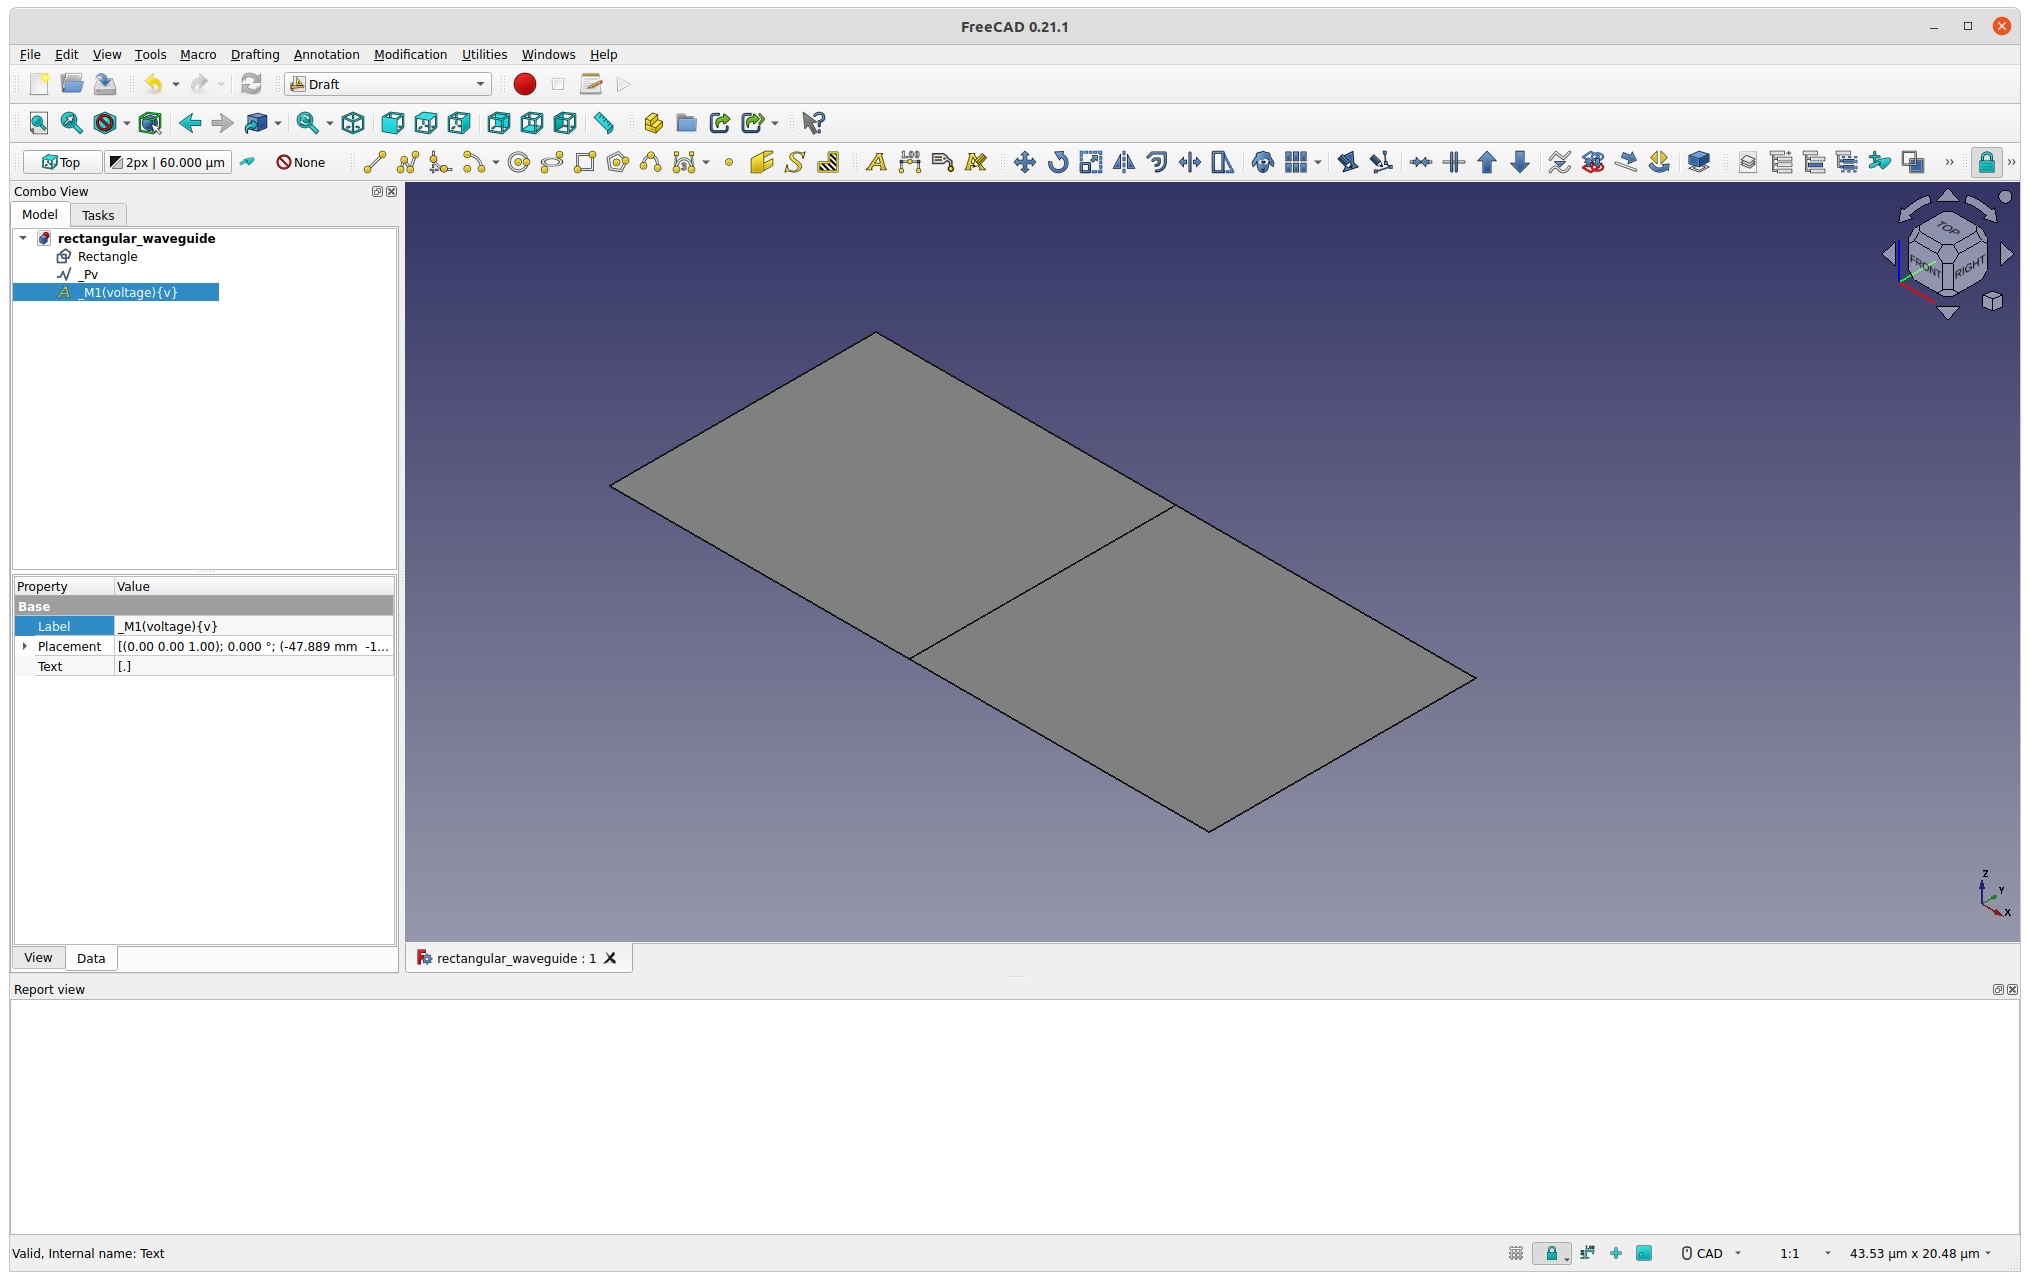
\includegraphics[width=0.75\textwidth]{../tutorials/OpenParEM2D/rectangular_waveguide/screenshots/rectangular_waveguide}
  \caption{Drawing and annotation for a WR90 rectangular waveguide.}
  \label{fig:rectangular_waveguide}
\end{figure}
\item Export the mode description file by selecting \texttt{Macro}$\rightarrow$\texttt{Macros ...}$\rightarrow$\texttt{OpenParEM2D\_save.py}$\rightarrow$\texttt{Execute}.  Enter the name \texttt{rectangular\_waveguide\_modes.txt}, then select \texttt{Save}.  Check the \texttt{Report view} window for errors.
\item Select the rectangle, then \texttt{File}$\rightarrow$\texttt{Export...}, make sure that the \texttt{BREP format} is selected, then save the file as \texttt{rectangular\_waveguide.brep}.
\item Save the drawing and exit FreeCAD.
\end{itemize}

\subsubsection{Meshing}

\begin{itemize}
\item Start gmsh as outlined in Sec.~\ref{sec:gmsh}.
\item Open the BREP file saved from the prior section by selecting \newline \texttt{File}$\rightarrow$\texttt{Open ...}$\rightarrow$\texttt{rectangular\_waveguide.brep}$\rightarrow$\texttt{Ok}.
\item Assign the material as air by clicking the options tree \newline$\boxplus$\texttt{Geometry}$\rightarrow$$\boxplus$\texttt{Physical Groups}$\rightarrow$$\boxplus$\texttt{Add}$\rightarrow$\texttt{Surface}.
\item In the pop-op window type \texttt{air} then select one of the crossing lines, which turns red.  Press the keyboard \texttt{e} and a new pop-up appears.  Click \texttt{Create new `.geo' file}.  Finally, press the keyboard \texttt{q} to finish.  [If the mouse does not select the dotted line, click the red box in the lower left to re-enable mouse input.]
\item To mesh the geometry, in the options tree click $\boxplus$\texttt{Mesh}$\rightarrow$\texttt{2D}. A screenshot of the mesh is shown in Fig.~\ref{fig:rectangular_mesh}.
\begin{figure}
  \centering
  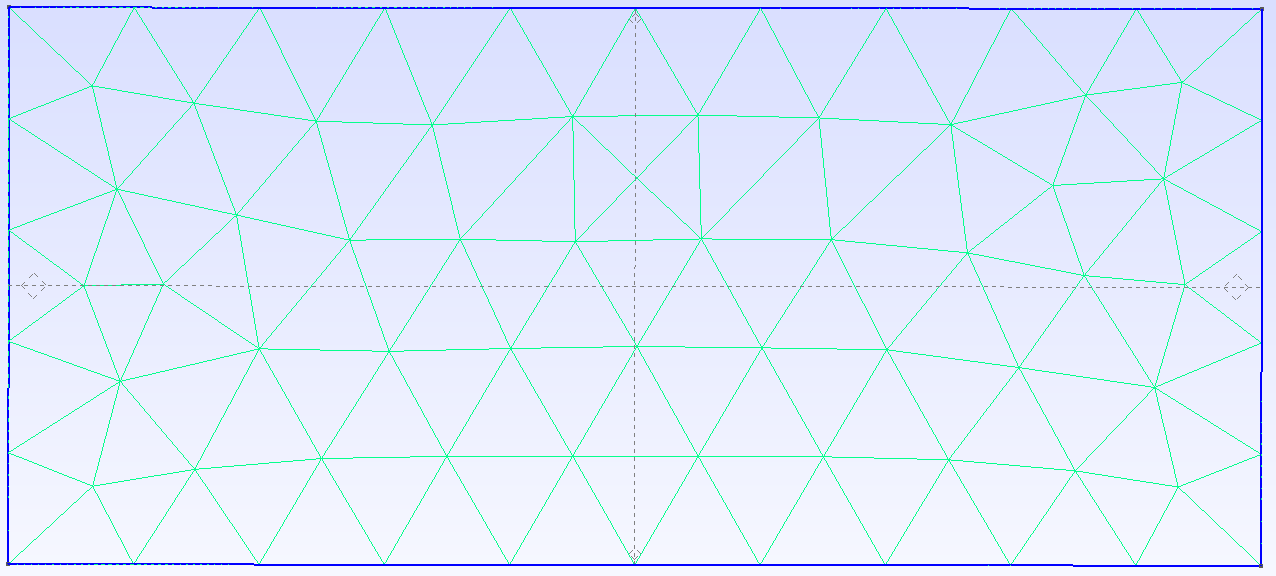
\includegraphics[width=0.4\textwidth]{../tutorials/OpenParEM2D/rectangular_waveguide/screenshots/rectangular_mesh}
  \caption{Screenshot of the meshed WR90 rectangular waveguide.}
  \label{fig:rectangular_mesh}
\end{figure}
\item Save the mesh by selecting \texttt{File}$\rightarrow$\texttt{Save Mesh}.
\item Quit gmsh.
\end{itemize}

\subsubsection{Solving}

\begin{itemize}

\item Create the materials file \texttt{global\_materials.txt} in any text editor and set the text contents to
\begin{Verbatim}[fontsize=\small]
  #OpenParEMmaterials 1.0
  Material
     name=air
     Temperature
        temperature=any
        Frequency
           frequency=any
           er=1.0006
           mur=1
           tand=0
           Rz=0
        EndFrequency
     EndTemperature
     Source
        Constantine A. Balanis, "Advanced Engineering Electromagnetics",
        John Wiley and Sons, 1989, p.79.
     EndSource
  EndMaterial
\end{Verbatim}
\item Create the project control file \texttt{rectangular\_waveguide.proj} in any text editor and set the text contents to
\begin{Verbatim}[fontsize=\small]
  #OpenParEM2Dproject 1.0
  project.save.fields            true
  mesh.file                      rectangular_waveguide.msh
  mesh.order                     3
  mode.definition.file           rectangular_waveguide_modes.txt
  materials.global.path          ./
  materials.global.name          global_materials.txt
  materials.local.path           ./
  materials.local.name           //local_materials.txt
  refinement.frequency           none
  frequency.plan.point           10e9
  solution.modes                 5
  solution.modes.buffer          10
  solution.impedance.definition  PV
  solution.impedance.calculation modal
\end{Verbatim}

\noindent Note that iterative refinement is not needed for this problem since the mesh is fairly dense, 3$^{\textnormal{rd}}$-order finite elements are used, and the fields vary slowly.  See Appendix~\ref{sec:control_file_spec} for a complete list of available keyword/value pairs that can be included in the project control file.

\item Run OpenParEM2D at the command line with
\begin{Verbatim}[fontsize=\small]
   $ OpenParEM2D rectangular_waveguide.proj
\end{Verbatim}
to run serially with a single core or with
\begin{Verbatim}[fontsize=\small]
   $ mpirun -q --oversubscribe -np 4 OpenParEM2D rectangular_waveguide.proj
\end{Verbatim}
to run in parallel with 4 cores.  Substitute a larger or smaller core number as needed.  The option \verb+--oversubscribe+ is not needed if the number of cores is less than or equal to half the number of available cores.
\end{itemize}

\subsubsection{Results}

The output includes the computed results
\begin{Verbatim}[fontsize=\scriptsize]
   -------------------------------------------------------------------------------------------------------------------------
    mode     frequency           er,eff       alpha,dB/m  beta/1000,rad/m          beta/ko         Zo(real)         Zo(imag)
   -------------------------------------------------------------------------------------------------------------------------
    1            1e+10        0.5706391   -1.0119426e-10       0.15832151       0.75540658        443.29902   -2.5441599e-11
    2            1e+10    5.1589308e-27        1543.8729    1.5053553e-14    7.1825698e-14
    3            1e+10    1.0011881e-27        1974.2013    6.6315799e-15    3.1641556e-14
    4            1e+10     2.237198e-27        2307.0205    9.9131431e-15    4.7299027e-14
    5            1e+10    1.3660112e-27        2307.0213   -7.7461569e-15   -3.6959588e-14
   -------------------------------------------------------------------------------------------------------------------------
\end{Verbatim}
\noindent showing 1 propagating mode and 4 cutoff higher-order modes.  Modes 4 and 5 are degenerate since they have the same complex propagation constant.  An impedance is generated only for mode 1 since a voltage integration line is only generated for modenumber=1.

From "rectangular\_waveguide\_results.csv", beta/ko for mode 1 is 0.755406579379436 vs. the exact analytical result of 0.755406579840748, so the OpenParEM2D result with this setup is accurate to 9 decimal places.  Alpha in dB/m for mode 2 is 1543.87289318585 vs. the exact analytical result of 1543.8726526439, so again a very close match.  The comparison is similar for the remaining 3 modes.  For the characteristic impedance for mode 1, the OpenParEM2D result is 443.299021764102~$\Omega$ vs. the exact analytical result of 443.299540513372~$\Omega$.

Note that the results change slightly from run-to-run.  This is due to the use of an iterative solution combined with MPI processing.

Fields can be viewed with ParaView as follows.
\begin{itemize}
\item Start ParaView at the command line with \verb+$ paraview &+, then navigate to and open the fields result \newline \texttt{rectangular\_waveguide\_frequency\_1e+10\_mode\_1.pvd}
\item Run \texttt{Macros}$\rightarrow$\texttt{field\_plot}.  Wait a few moments.
\item A wide variety of plots are available for viewing, both magnitude and vector.
\item Scaling in ParaView does not work well for vector plots, so manual adjustment is always required.
\item Click \texttt{E real vector} then enter 2e-6 for \texttt{Scale Factor}.
\item The resulting field plot is shown in Fig.~\ref{fig:rectangular_ReEt}, where the electric field is vertically directed.
\begin{figure}[H]
  \centering
  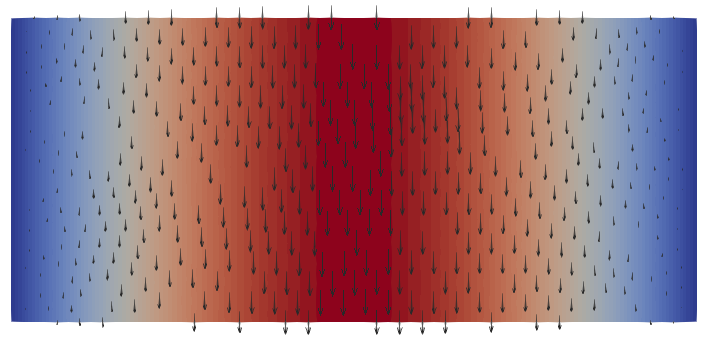
\includegraphics[width=0.4\textwidth]{../tutorials/OpenParEM2D/rectangular_waveguide/screenshots/rectangular_ReEt}
  \caption{Re($Et$) for the WR90 rectangular waveguide.}
  \label{fig:rectangular_ReEt}
\end{figure}
\end{itemize}


\subsection{Coaxial Waveguide}

RG401 type 0.250 semi-rigid coaxial cable is constructed, annotated, meshed, and solved.  The RG401 coax is assumed to have an inner conductor diameter of 1.63~mm, an outer conductor inner diameter of 5.46~mm, a PTFE dielectric with $\epsilon_r=2.1$ and a $\textnormal{tan}\delta=0.0004$.  The metals are assumed to be copper with $\sigma=5.813\times 10^7$ S/m.

\subsubsection{Drawing and Mode Annotation}

\begin{itemize}
\item Create a directory for the project
\begin{Verbatim}[fontsize=\small]
$ mkdir coaxial_waveguide
$ cd coaxial_waveguide
\end{Verbatim}
\item Start FreeCAD, open a new drawing, set preferences [if needed], set the drawing workspace to \texttt{Draft}, and set the drawing plane to \texttt{Top} as outlined in Sec.~\ref{sec:freecad}.
\item Click \texttt{Drafting}$\rightarrow$\texttt{Polygon} or click on the polygon icon on the toolbar and draw a polygon of any size by clicking to start then clicking to end.  This is the first polygon.
\item Select the polygon either on the drawing space or in the \texttt{Combo View} window.
\item In the \texttt{Property} window, for property \texttt{Radius} change the value to 0.815~um.  Sec.~\ref{sec:freecad} discusses why drawings are in $\mu$m to ultimately obtain a mesh in mm.  Change the property \texttt{Faces Number} to 36. This is the center conductor.
\item Again in the \texttt{Property} window, navigate through the properties \texttt{Placement}$\rightarrow$\texttt{Position} then enter 0 for x, y, and z.
\item Zoom to view the polygon  with \texttt{View}$\rightarrow$\texttt{Standard Views}$\rightarrow$\texttt{Fit All}.
\item On the toolbar, click the $\gg$ to show the snap options, and click \texttt{Snap Center}.
\item Draw a second polygon snapped to the center of the first and configure it with the same settings so that it is a copy.  Alternatively, copy the the first polygon to a second with the \texttt{Copy} and \texttt{Paste} commands under the \texttt{Edit} menu command.  Do not use a cloned object because the Python script \texttt{OpenParEM2D\_save.py} does not support clones.
\item Change the Label property of the second polygon to \texttt{\_Pinner}.  Change the property \texttt{Make Face} to false [optional, but looks better]. This path is used for both the current integration path and the surface impedance boundary using copper for the center conductor.
\item Draw a third polygon snapped to the center of the first with the same settings except with a radius of 2.73~um.  This is the dielectric once the center conductor is removed.
\item Copy and paste the third polygon to a fourth and change its Label property to \texttt{\_Pouter}.  Set its property \texttt{Make Face} to false, if desired.  This path is used for the surface impedance boundary using copper for the outer conductor.
\item Change the drawing workspace to \texttt{Part}.  Select the third polygon then the first, then select \newline\texttt{Part}$\rightarrow$\texttt{Boolean}$\rightarrow$\texttt{Cut} to cut the center conductor from the dielectric.  Agree to the operation in the warning pop-up window.  This object is the coax.  Change the Label property to \texttt{coax}.
\item Change the drawing workspace back to \texttt{Draft}.
\item Draw a line from the outer conductor of the coaxial cable to the inner conductor.  Change its Label to \newline\texttt{\_Pv}.  This is the integration path for the voltage.
\item Add a text object with the Label \texttt{\_M1(voltage)\{v\}}.  This is the modal definition for the voltage.
\item Add a text object with the Label \texttt{\_M1(current)\{inner\}}.  This is the modal definition for the current.
\item Add a text object with the Label \texttt{\_Bi(SI,copper)\{inner\}}.  This is the surface impedance definition for the inner conductor.
\item Add a text object with the Label \texttt{\_Bo(SI,copper)\{outer\}}.  This is the surface impedance definition for the outer conductor.
\item Save the drawing with the name \texttt{coaxial\_waveguide} using \texttt{File}$\rightarrow$\texttt{Save}.
\item The completed drawing and annotation is shown in Fig.~\ref{fig:coaxial_drawing}, where the \texttt{\_Pinner} is highlighted in green and \texttt{\_Pouter} is highlighted in yellow.
\begin{figure}
  \centering
  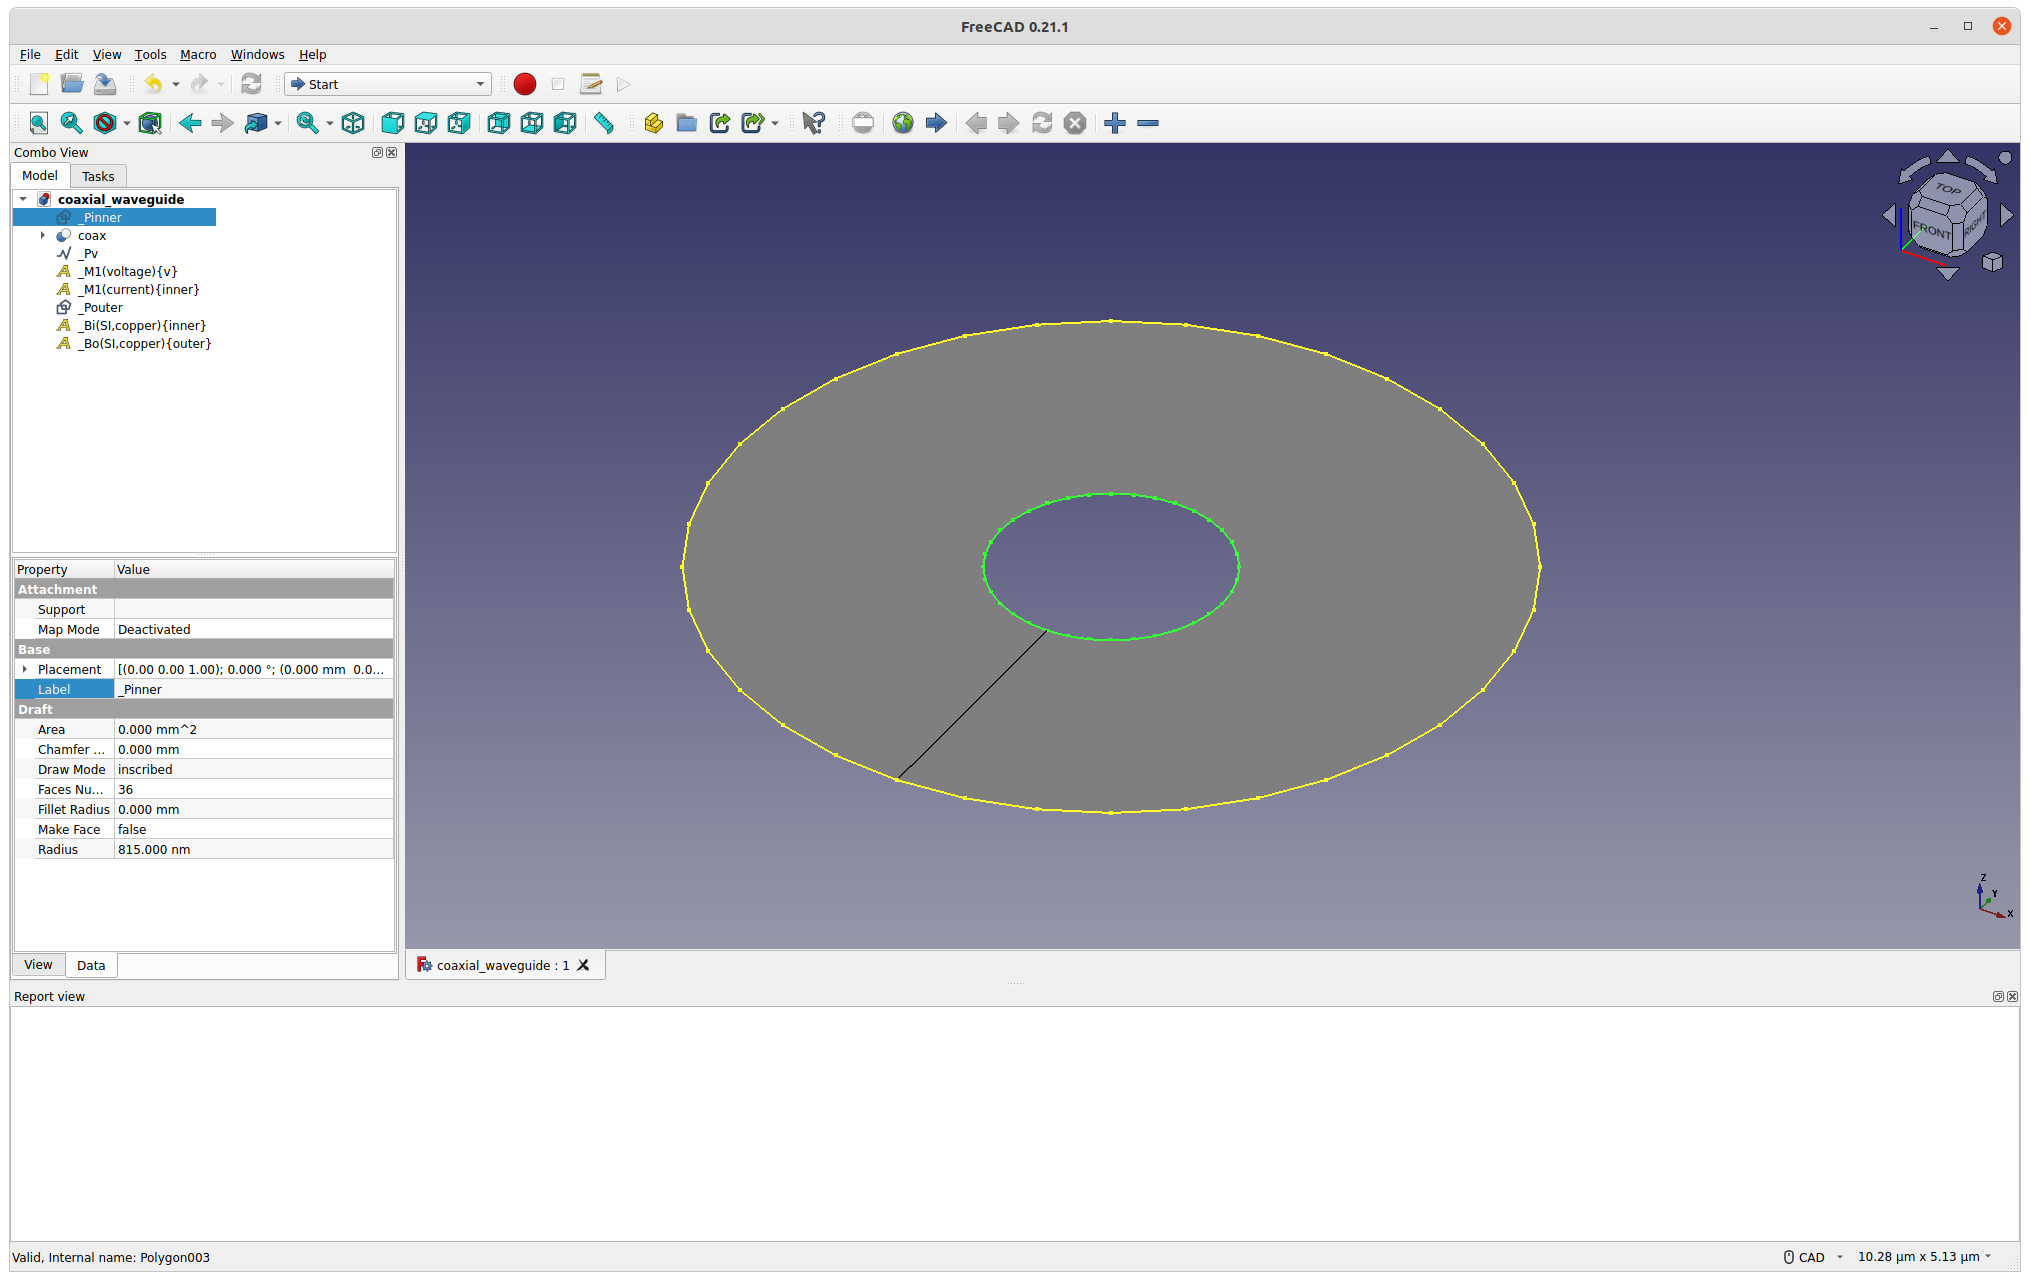
\includegraphics[width=0.75\textwidth]{../tutorials/OpenParEM2D/coaxial_waveguide/screenshots/coaxial_drawing}
  \caption{Drawing and annotation for an RG401 coaxial waveguide.}
  \label{fig:coaxial_drawing}
\end{figure}
\item Export the mode description file by selecting \texttt{Macro}$\rightarrow$\texttt{Macros ...}$\rightarrow$\texttt{OpenParEM2D\_save.py}$\rightarrow$\texttt{Execute}.  Enter the name \texttt{coaxial\_waveguide\_modes.txt}, then select \texttt{Save}.  Check the \texttt{Report view} window for errors.
\item Select the \texttt{coax} object, then \texttt{File}$\rightarrow$\texttt{Export...}, make sure that the \texttt{BREP format} is selected, then save the file as \texttt{coaxial\_waveguide.brep}.
\item Save the drawing and exit FreeCAD.
\end{itemize}

\subsubsection{Meshing}

\begin{itemize}
\item Start gmsh as outlined in Sec.~\ref{sec:gmsh}.
\item Open the BREP file saved from the prior section by selecting \newline \texttt{File}$\rightarrow$\texttt{Open ...}$\rightarrow$\texttt{coaxial\_waveguide.brep}$\rightarrow$\texttt{Ok}.
\item Assign the material as PTFE by clicking the options tree \newline$\boxplus$\texttt{Geometry}$\rightarrow$$\boxplus$\texttt{Physical Groups}$\rightarrow$$\boxplus$\texttt{Add}$\rightarrow$\texttt{Surface}.
\item In the pop-op window type \texttt{PTFE} then select one of the crossing lines, which turns red.  Press the keyboard \texttt{e} and a new pop-up appears.  Click \texttt{Create new `.geo' file}.  Finally, press the keyboard \texttt{q} to finish.  [If the mouse does not select the dotted line, click the red box in the lower left to re-enable mouse input.]
\item To mesh the geometry, in the options tree click $\boxplus$\texttt{Mesh}$\rightarrow$\texttt{2D}. A screenshot of the mesh is shown in Fig.~\ref{fig:coaxial_mesh}.
\begin{figure}
  \centering
  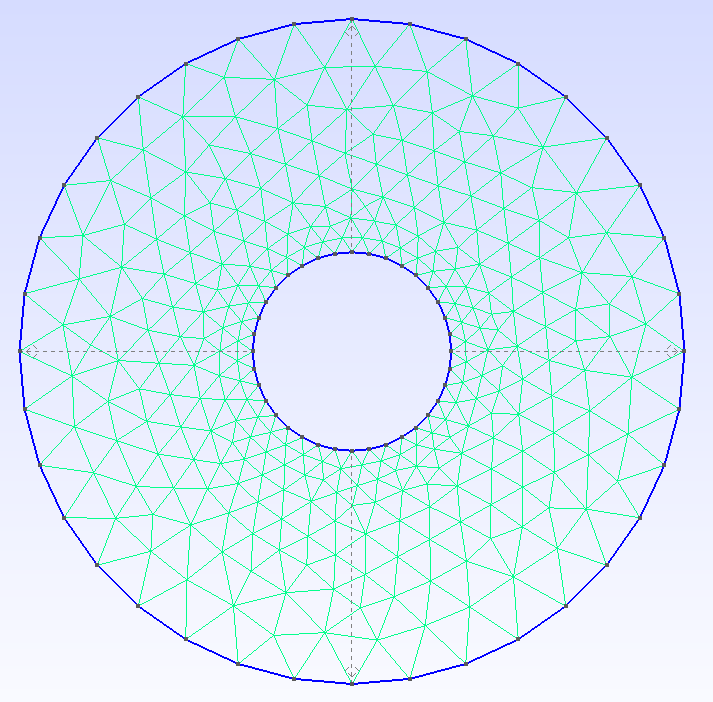
\includegraphics[width=0.4\textwidth]{../tutorials/OpenParEM2D/coaxial_waveguide/screenshots/coaxial_mesh}
  \caption{Screenshot of the meshed RG401 coaxial waveguide.}
  \label{fig:coaxial_mesh}
\end{figure}
\item Save the mesh by selecting \texttt{File}$\rightarrow$\texttt{Save Mesh}.
\item Quit gmsh.
\end{itemize}

\subsubsection{Solving}

\begin{itemize}

\item Create the materials file \texttt{local\_materials.txt} in any text editor and set the text contents to
\begin{Verbatim}[fontsize=\small]
  #OpenParEMmaterials 1.0
  Material
     name=PTFE
     Temperature
        temperature=any
        Frequency
           frequency=any
           er=2.1
           mur=1
           tand=0.0004
           Rz=0
        EndFrequency
     EndTemperature
     Source
        generic numbers
     EndSource
  EndMaterial
  Material
     name=copper
     Temperature
        temperature=20
        Frequency
           frequency=any
           er=1
           mur=1
           conductivity=5.813e7
           Rz=0
        EndFrequency
     EndTemperature
     Source
        David M. Pozar, "Microwave Engineering," Addison-Wesley Publishing Company,
           1990, p.714.
     EndSource
  EndMaterial
\end{Verbatim}
\item Create the project control file \texttt{coaxial\_waveguide.proj} in any text editor and set the text contents to
\begin{Verbatim}[fontsize=\small]
  #OpenParEM2Dproject 1.0
  project.save.fields            true
  mesh.file                      coaxial_waveguide.msh
  mesh.order                     3
  mode.definition.file           coaxial_waveguide_modes.txt
  materials.global.path          ./
  materials.global.name          //global_materials.txt
  materials.local.path           ./
  materials.local.name           local_materials.txt
  refinement.frequency           none
  frequency.plan.point           10e9
  solution.modes                 1
  solution.modes.buffer          0
  solution.impedance.definition  PV
  solution.impedance.calculation modal
  solution.temperature           20
  debug.show.impedance.details   true
\end{Verbatim}

\noindent Note that iterative refinement is not needed for this problem since the mesh is fairly dense, 3$^{\textnormal{rd}}$-order finite elements are used, and the fields vary slowly.  See Appendix~\ref{sec:control_file_spec} for a complete list of available keyword/value pairs that can be included in the project control file.

\item Run OpenParEM2D at the command line with
\begin{Verbatim}[fontsize=\small]
   $ OpenParEM2D coaxial_waveguide.proj
\end{Verbatim}
to run serially with a single core or with
\begin{Verbatim}[fontsize=\small]
   $ mpirun -q --oversubscribe -np 4 OpenParEM2D coaxial_waveguide.proj
\end{Verbatim}
to run in parallel with 4 cores.  Substitute a larger or smaller core number as needed.  The option \verb+--oversubscribe+ is not needed if the number of cores is less than or equal to half the number of available cores.
\end{itemize}

\subsubsection{Results}

The output includes the characteristic impedance computed with all three definitions, shown as
\begin{Verbatim}
   Mode
        1  voltage (V): (5.13256,9.54287e-12)
           current (I): (0.102229,-2.04457e-05)
           Pz (Pz,avg): (0.263587,5.27173e-05)
   Mode
        1  Impedance (VI): (50.2067,0.0100413)
                     (PV): (49.9706,0.00999411)
                     (PI): (50.4439,0.0100888)
\end{Verbatim}
The PV definition is very close to the designed value of 50~$\Omega$. The output also includes the computed results
\begin{Verbatim}[fontsize=\scriptsize]
   -------------------------------------------------------------------------------------------------------------------------
    mode     frequency           er,eff       alpha,dB/m  beta/1000,rad/m          beta/ko         Zo(real)         Zo(imag)
   -------------------------------------------------------------------------------------------------------------------------
    1            1e+10        2.1000001        1.0990629        0.3037168        1.4491377         49.97056     0.0099941114
   -------------------------------------------------------------------------------------------------------------------------
\end{Verbatim}
\noindent showing the effective dielectric constant as 2.1000001, which is very close to the lossless theoretical value of 2.1 for this homogeneous material.

The loss is 1.099~dB/m. Fairview Microwave on its datasheet for RG401 Type 0.250 part number FM-SR250CU-STR specifies the loss as 1.083~dB/m.  These two loss figures are in very good agreement given that the exact dimensions nor material properties of the Fairview Microwave product are known.  Simply using generic numbers gets very close.

Note that the results change slightly from run-to-run.  This is due to the use of an iterative solution combined with MPI processing.

Fields can be viewed with ParaView as follows:
\begin{itemize}
\item Start ParaView at the command line with \verb+$ paraview &+, then navigate to and open the fields result \newline \texttt{coaxial\_waveguide\_frequency\_1e+10\_mode\_1.pvd}
\item Run \texttt{Macros}$\rightarrow$\texttt{field\_plot}.  Wait a few moments.
\item A wide variety of plots are available for viewing, both magnitude and vector.
\item Disable all plots then enable \texttt{Ht real magnitude} and \texttt{H real vector}.
\item Click \texttt{H real vector} then enter 1e-5 for \texttt{Scale Factor}.
\item The resulting field is shown in Fig.~\ref{fig:coaxial_ReHt}, where the magnetic field circles the center conductor.
\begin{figure}[H]
  \centering
  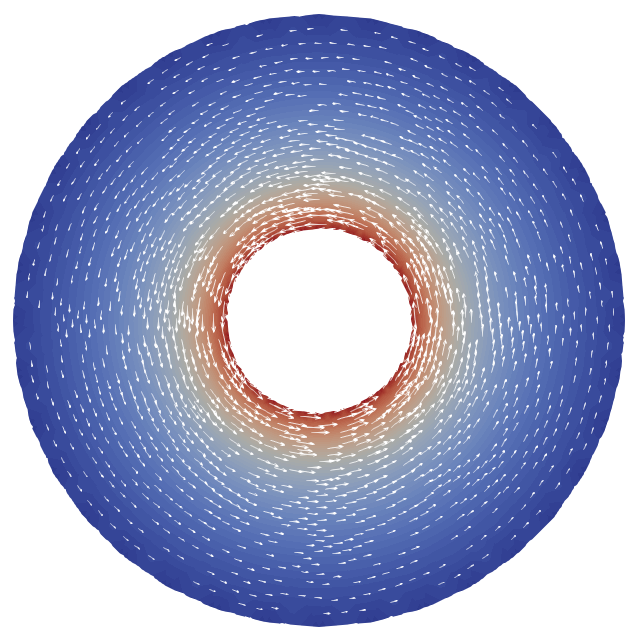
\includegraphics[width=0.4\textwidth]{../tutorials/OpenParEM2D/coaxial_waveguide/screenshots/coaxial_ReHt}
  \caption{Re($Ht$) for the RG401 coaxial waveguide.}
  \label{fig:coaxial_ReHt}
\end{figure}
\end{itemize}

\subsection{Coupled Microstrip with Line Setup}
\label{sec:coupled_microstrip}

The coupled microstrip pair from Fig.~8 in \cite{Olyslager} is set up with line integration paths and solved for the even and odd characteristic impedances and propagation constants.

\subsubsection{Drawing and Mode Annotation}

\begin{itemize}
\item As for the prior tutorials, start a new project called \texttt{coupled\_microstrip} with a new drawing in FreeCAD with the drawing plane set to \texttt{Top}.
\item Draw a rectangle 1~um wide and 0.3~um tall [to ultimately result in 1 and 0.3~mm], and set the placement to x=-1.5~um and y=0.  Zoom to fit. Set Label to \texttt{cut1}.
\item Select the rectangle and copy it using \texttt{Edit}$\rightarrow$\texttt{Copy} then \texttt{Edit}$\rightarrow$\texttt{Paste}.  Set Label to \texttt{\_Pi1}.  This is the current integration path for the first microstrip line.
\item Select object \texttt{\_Pi1} and copy it.  Set the placement to x=0.5~um and y=0. Change Label to \texttt{cut2}.
\item Select object \texttt{cut2} and copy it.  Set Label to \texttt{\_Pi2}.  This is the current integration line for the second microstrip line.
\item Select object \texttt{\_Pi2} and copy it.  Set Label to \texttt{substrate}. Set Height to 0.635~um and the width to 10~um.  Set the position to x=-5~um and y=-0.635~um.
\item Select object \texttt{substrate} and copy it.  Set Label to \texttt{air}.  Set Height to 3~um. Set the position with y=0.
\item Set the drawing workspace to \texttt{Part}.
\item Select \texttt{air} then \texttt{cut1}, then select \texttt{Part}$\rightarrow$\texttt{Boolean}$\rightarrow$\texttt{Cut}.  Click \texttt{Yes} in the pop-up.
\item Select the cut object then \texttt{cut2} and repeat the Boolean cut operation. Set Label to \texttt{air-metal}.  The rectangular voids form the microstrip lines since all edges next to void spaces default to PEC.
\item Select \texttt{View}$\rightarrow$\texttt{Visibility}$\rightarrow$\texttt{Hide all objects}.
\item Save the drawing as \texttt{coupled\_microstrip}.
\item Select \texttt{substrate} and \texttt{air-metal} and press the space bar to view the objects.
\item Set the drawing workspace to \texttt{Draft}. 
\item Set snap options to include \texttt{Snap Midpoint}.
\item Draw a line from the center at the bottom of \texttt{substrate} to the center at the top of \texttt{substrate}.  Set Label to \texttt{\_Pv1}. Set the position to x=-1~um.  This is the voltage integration line for the first microstrip line.
\item Copy \texttt{\_Pv1}, set Label to \texttt{\_Pv2}, and set the position x=1~um.  This is the voltage integration line for the second microstrip line.
\item Add a text object with the Label \texttt{\_L1(voltage)\{v1\}}.  This is the line definition for the voltage on the first microstrip.
\item Add a text object with the Label \texttt{\_L2(voltage)\{v2\}}.  This is the line definition for the voltage on the second microstrip.
\item Add a text object with the Label \texttt{\_L1(current)\{i1\}}.  This is the line definition for the current on the first microstrip.
\item Add a text object with the Label \texttt{\_L2(current)\{i2\}}.  This is the line definition for the current on the second microstrip.
\item The drawing should look like that in Fig.~\ref{fig:coupled_drawing}, showing the substrate and air above the substrate along with the voltage integration lines.
\begin{figure}[H]
  \centering
  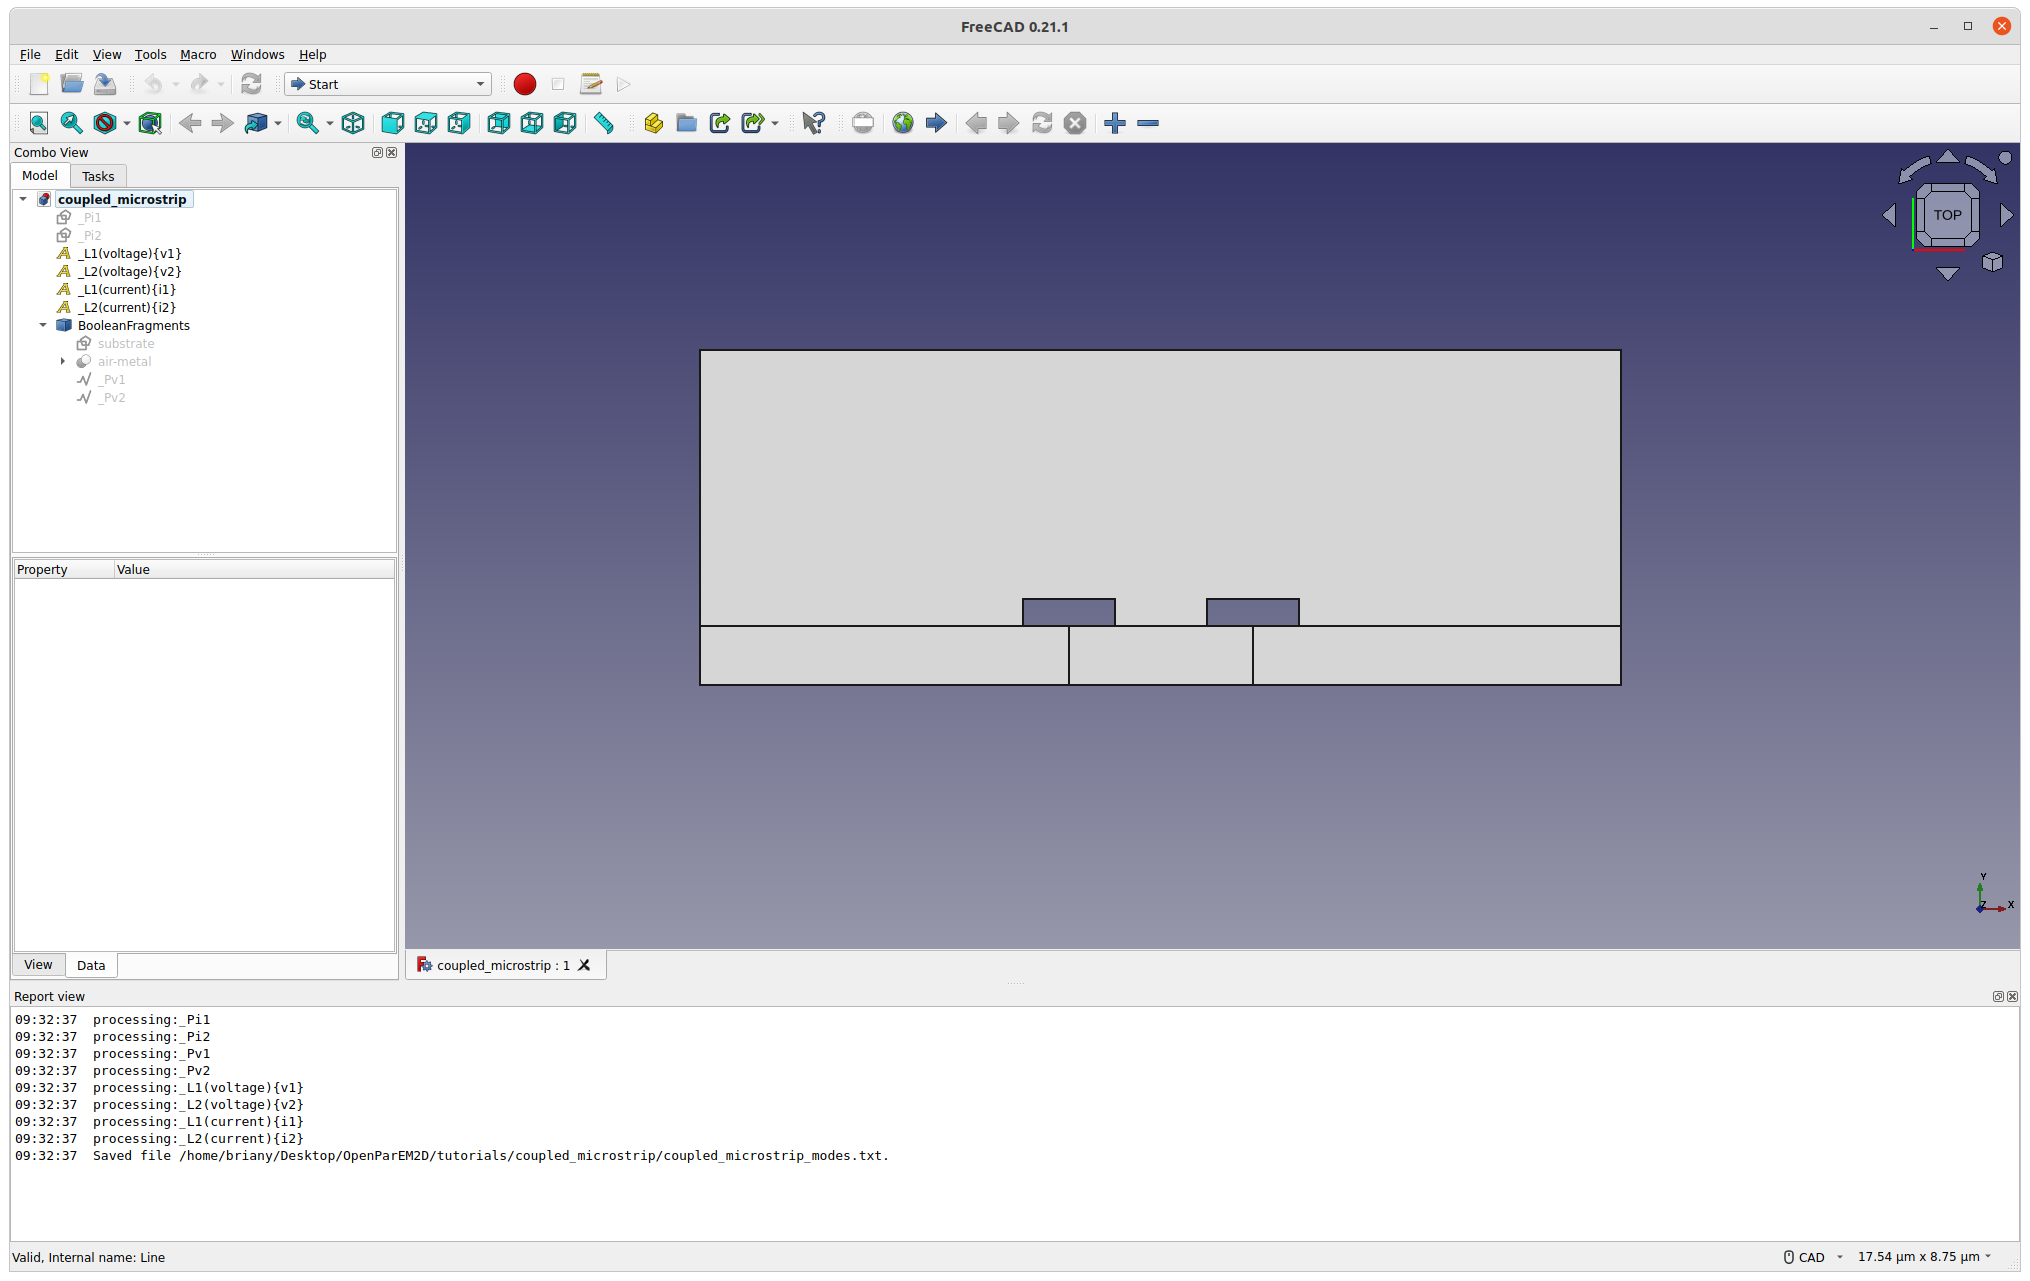
\includegraphics[width=0.75\textwidth]{../tutorials/OpenParEM2D/coupled_microstrip/screenshots/coupled_drawing}
  \caption{Coupled microstrip with annotations.}
  \label{fig:coupled_drawing}
\end{figure}
\item Set the drawing workspace to \texttt{Part}.
\item Select \texttt{substrate}, \texttt{air-metal}, \texttt{\_Pv1}, and \texttt{\_Pv2}, then select \texttt{Part}$\rightarrow$\texttt{Split}$\rightarrow$\texttt{Boolean Fragments}. By including the voltage integration lines, gmsh will include these an an edge in the mesh.
\item Execute the macro \texttt{OpenParEM2D\_save.py} to save the mode description file as \texttt{coupled\_microstrip\_modes.txt}.
\item Save the drawing and exit FreeCAD.
\end{itemize}

\subsubsection{Meshing}

\begin{itemize}
\item Start gmsh and open the saved BREP file.
\item Assign physical groups \texttt{air} to the surface representing air and \texttt{alumina} to the surface representing the substrate using the \texttt{Add Surface} methodology described in the prior tutorials.
\item Mesh for 2D then save the mesh.
\item Quit gmsh.

\end{itemize}

\subsubsection{Solving}

\begin{itemize}
\item Create the materials file \texttt{local\_materials.txt} and set the text contents to
\begin{Verbatim}[fontsize=\small]
  #OpenParEMmaterials 1.0
  Material
     name=air
     Temperature
        temperature=any
        Frequency
           frequency=any
           er=1.0006
           mur=1
           tand=0
           Rz=0
        EndFrequency
     EndTemperature
     Source
        Constantine A. Balanis, "Advanced Engineering Electromagnetics",
        John Wiley and Sons, 1989, p.79.
     EndSource
  EndMaterial
  Material
     name=alumina
     Temperature
        temperature=any
        Frequency
           frequency=any
           er=9.8
           mur=1
           tand=0
           Rz=0
        EndFrequency
     EndTemperature
     Source
     EndSource
  EndMaterial
\end{Verbatim}
\item Create the project control file \texttt{coupled\_microstrip.proj} set the text contents to
\begin{Verbatim}[fontsize=\small]
  #OpenParEM2Dproject 1.0
  project.save.fields            true
  mesh.file                      coupled_microstrip.msh
  mesh.order                     4
  mesh.refinement.fraction       0.01
  mode.definition.file           coupled_microstrip_modes.txt
  materials.global.path          ./
  materials.global.name          //global_materials.txt
  materials.local.path           ./
  materials.local.name           local_materials.txt
  refinement.frequency           high
  frequency.plan.point           40.11e9
  refinement.variable            |Zo|
  refinement.iteration.min       1
  refinement.iteration.max       40
  refinement.required.passes     1
  refinement.tolerance           0.0001
  solution.modes                 2
  solution.modes.buffer          0
  solution.impedance.definition  PI
  solution.impedance.calculation line
  debug.show.impedance.details   true
\end{Verbatim}
\item Run OpenParEM2D with the proj file.
\end{itemize}

\subsubsection{Results}

OpenParEM2D calculates the characteristic impedances for common and differential modes, while \cite{Olyslager} quotes results for the even and odd modes.  To compare, the OpenParEM2D results are converted so that the even mode characteristic impedance is calculated as twice the common mode impedance, while the odd mode impedance is half the differential impedance.  The results are shown in Table~\ref{table:coupled_results}, where the \cite{Olyslager} results are scaled off the printed plot.  The results are in excellent agreement with a small difference in the odd mode characteristic impedance.

\begin{table}[ht]
\caption{Comparison of Results}
\begin{center}
\begin{tabular}{|c|c|c|}
\hline
Characteristic & Simulation of \cite{Olyslager} & OpenParEM2D \\
\hline
$\beta_e/k_\circ$ & 2.93 & 2.94 \\
$\beta_o/k_\circ$ & 2.82 & 2.82 \\
$Z_{\circ e},\Omega$ & 50.8 & 50.6 \\
$Z_{\circ o},\Omega$ & 43.4 & 42.6 \\
\hline
\end{tabular}
\end{center}
\label{table:coupled_results}
\end{table}

Due to the sharp corners on the microstrip lines, adaptive mesh refinement is used in this solution.  The initial and final refined meshes are shown in Fig.~\ref{fig:coupled_mesh}, where the refinement concentrates on the corners and the dielectric interface.

\begin{figure}[H]
  \centering
  \begin{subfigure}{0.45\textwidth}
     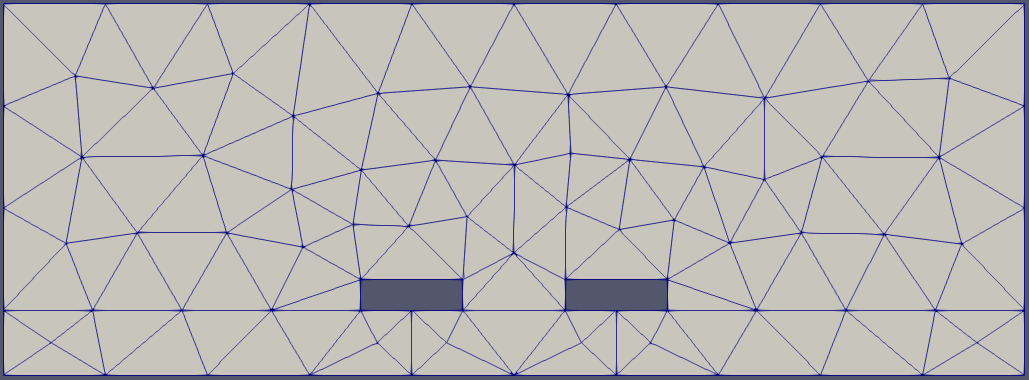
\includegraphics[width=\linewidth]{../tutorials/OpenParEM2D/coupled_microstrip/screenshots/coupled_initial_mesh}
     \caption{Initial mesh as produced by gmsh.}
  \end{subfigure}
  \begin{subfigure}{0.45\textwidth}
     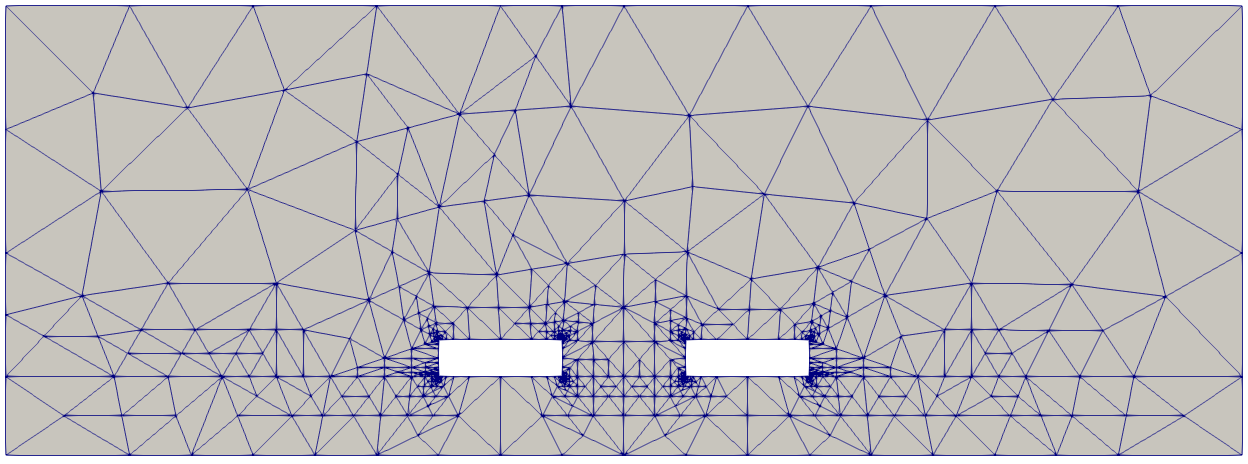
\includegraphics[width=\linewidth]{../tutorials/OpenParEM2D/coupled_microstrip/screenshots/coupled_refined_mesh}
     \caption{Refined mesh after 26 iterations.}
  \end{subfigure}
  \caption{Initial and refined meshes for the coupled microstrip lines.}
  \label{fig:coupled_mesh}
\end{figure}

The fields can be viewed with ParaView, where pre-configured plots are generated using the macro \texttt{field\_plot}.  Plots for the common and differential modes are shown in Fig.~\ref{fig:coupled_fields}.  In these plots, the background shows $\textnormal{Re}(|\overline{E}|)$, while the black vectors show $\textnormal{Re}(\overline{E})$ and the white vectors show $\textnormal{Re}(\overline{H})$. Note that $\textnormal{Re}(\overline{E})$ and $\textnormal{Re}(\overline{H})$ do not use the same scale.

\begin{figure}[H]
  \centering
  \begin{subfigure}{0.75\textwidth}
     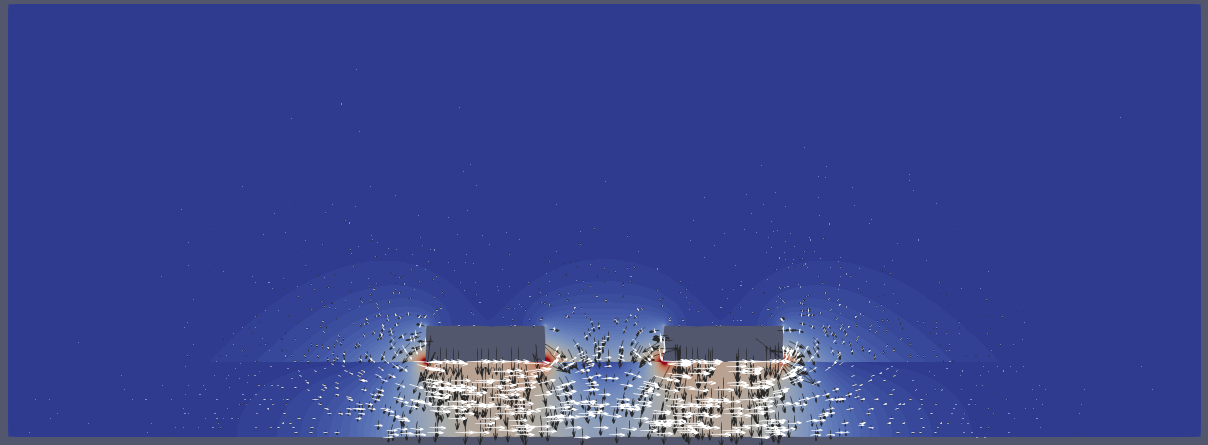
\includegraphics[width=\linewidth]{../tutorials/OpenParEM2D/coupled_microstrip/screenshots/coupled_common_mode}
     \caption{Common mode.}
  \end{subfigure}
  \par\bigskip
  \begin{subfigure}{0.75\textwidth}
     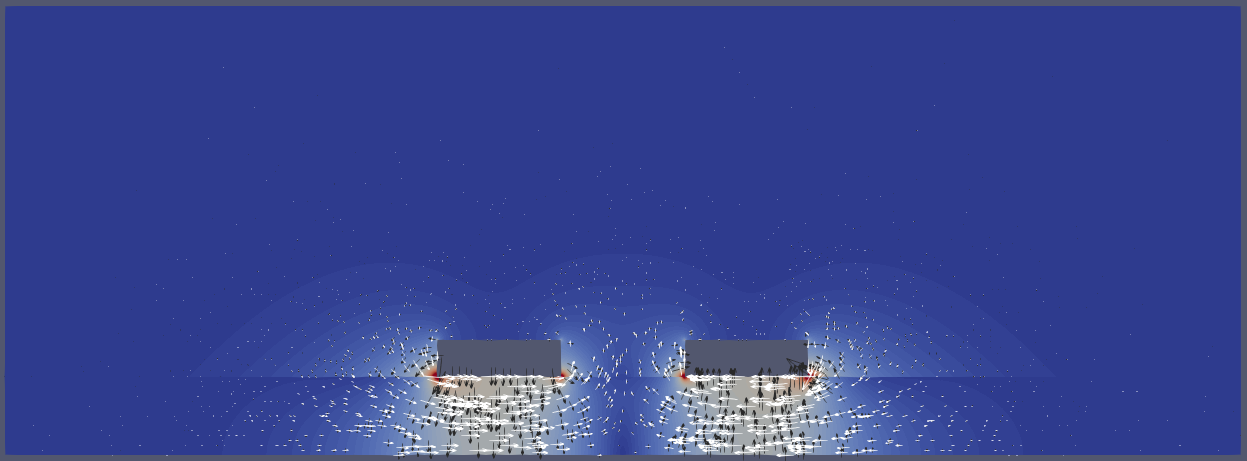
\includegraphics[width=\linewidth]{../tutorials/OpenParEM2D/coupled_microstrip/screenshots/coupled_differential_mode}
     \caption{Differential mode.}
  \end{subfigure}
  \caption{Plots of the common-mode and differential-mode fields.}
  \label{fig:coupled_fields}
\end{figure}

\subsection{Coupled Microstrip with Modal Setup}

The tutorial from Sec.~\ref{sec:coupled_microstrip} is re-worked using modal setups for the voltage and current integration paths.  The setups are nearly identical, so just the changes are discussed.

\subsubsection{Drawing and Mode Annotation}

\begin{itemize}
\item Copy the tutorial project directory from \texttt{coupled\_microstrip} to \texttt{coupled\_microstrip\_modal}.
\item In FreeCAD, change \texttt{\_L1(voltage)\{v1\}} to \texttt{\_M1(voltage,0.5)\{v1,v2\}}.  Mode 1 is the common-mode mode, so the voltages on the lines are equal due to symmetry.  The modified annotation has OpenParEM2D integrate along both paths, so the voltages is 2$\times$ too high, so a scaling factor of 0.5 is applied.
\item Change \texttt{\_L2(voltage)\{v2\}} to \texttt{\_M2(voltage)\{v1,-v2\}}.  Mode 2 is the differential mode, so the voltages are equal and opposite.  The modified annotation has OpenParEM2D integrate along the v1 path and then the v2 path in the reversed direction.  The total voltage is then found without need for a scaling factor.
\item Change \texttt{\_L1(current)\{i1\}} to \texttt{\_M1(current)\{i1,i2\}}.  For the common mode, the total current is the sum of the currents on the two lines.
\item Change \texttt{\_L2(current)\{i2\}} to \texttt{\_M2(current,0.5)\{i1,-i2\}}.  For the differential mode, the currents are equal and opposite.  The modified annotation has OpenParEM2D calculate the total currents on both lines then applies a scaling factor of 0.5.
\item Execute the macro \texttt{OpenParEM2D\_save.py} to save the mode description file as \texttt{coupled\_microstrip\_modes.txt}.
\item Save the drawing and exit FreeCAD.
\end{itemize}

\subsubsection{Meshing}

The existing mesh is re-used.

\subsubsection{Solving}

In the proj file, change the value for the keyword \texttt{solution.impedance.calculation} from \texttt{line} to \texttt{modal}.  Run OpenParEM2D.

\subsubsection{Results}

After 26 iterations, the results shown to the terminal are
\begin{Verbatim}[fontsize=\scriptsize]
   -------------------------------------------------------------------------------------------------------------------------
    mode     frequency           er,eff       alpha,dB/m  beta/1000,rad/m          beta/ko         Zo(real)         Zo(imag)
   -------------------------------------------------------------------------------------------------------------------------
    1        4.011e+10        8.6544292    2.1815834e-11        2.4730394        2.9418411        25.279915    2.7033135e-14
    2        4.011e+10        7.9720613    1.3477717e-11        2.3735432        2.8234839        85.178997    3.0707696e-14
   -------------------------------------------------------------------------------------------------------------------------
\end{Verbatim}
\noindent A run from the line setup [also after 26 iterations] in Sec.~\ref{sec:coupled_microstrip} shows nearly identical results as
\begin{Verbatim}[fontsize=\scriptsize]
   -------------------------------------------------------------------------------------------------------------------------
    mode     frequency           er,eff       alpha,dB/m  beta/1000,rad/m          beta/ko         Zo(real)         Zo(imag)
   -------------------------------------------------------------------------------------------------------------------------
    1        4.011e+10        8.6544292    -4.079956e-11        2.4730394        2.9418411        25.279915   -4.2724076e-14
    2        4.011e+10        7.9720613    7.4035296e-12        2.3735432        2.8234839        85.127309    4.7404632e-14
   -------------------------------------------------------------------------------------------------------------------------
\end{Verbatim}
\noindent where the only differences are the very minor changes due to the iterative nature of the solution interacting with MPI processing.

Impedance calculations are a post-processing step, so the field solution is the same for both setups.  The differences are simply that the line setup calculates voltages and currents on partial paths then combines them to get final values, while the modal setup calculates voltages and currents on total paths to get final values without further processing.  The two techniques must necessarily get the same results.

\section{Techniques}

\subsection{Finite Element Order}

The finite element order is set with the keyword/value pair \texttt{mesh.order N} in the project control file.  \texttt{N} can be any integer and sets the order of the polynomial approximating the field in each finite element.  All elements in a mesh have the same element order.

Higher values for \texttt{N} have potential advantages due to the polynomial accommodating larger field variations within any given element.  The advantages of higher order include:
\begin{itemize}
\item Greater accuracy for a given mesh size.
\item Smaller mesh size for a given accuracy.
\item Better accuracy for frequency sweeps.
\item Smoother fields for visualization.
\end{itemize}
\noindent However, there are also disadvantages of higher order:
\begin{itemize}
\item Slower run times for a given mesh size.
\item Larger memory consumption.
\item Slower mesh error calculation for a given mesh size.
\item Harder convergence for the initial solution, although order-ramping may offer a fix, when implemented.
\end{itemize}
\noindent The disadvantages ramp quickly with increasing \texttt{N}.
OpenParEM2D does not currently support GPU computing, which can alleviate the disadvantages of higher \texttt{N}.

Experience to date suggests the following guidelines for selecting \texttt{N}:
\begin{itemize}
\item Assuming a simulation runs to completion in an acceptable time, higher \texttt{N} is always better than lower \texttt{N}.
\item Avoid \texttt{N=1}.  Adaptive refinement is required and the number of iterations is just too great.  Improved adaptive meshing algorithms might address this issue.
\item Generally, \texttt{N=3} and \texttt{N=4} are good options.
\item Choose the largest \texttt{N} that allows a quick first iteration when using adaptive refinement.  What qualifies as \textit{quick} depends on mesh size.
\item In the first iteration, if it take more than a few seconds or requires a very large iteration limit [like 100,000], then decrease \texttt{N}.  Conversely, if the first iteration is very quick, then try increasing \texttt{N}.  Note that very slow convergence can be caused by poor mesh quality, so it is important to ensure that the mesh has good triangulation by avoiding long thin triangles.
\item Problems with relatively smooth fields, such as those using waveguide, greatly benefit from larger \text{N}.  For some problems, adaptive refinement may not be needed.
\item Problems with sharp edges, such as edge-coupled stripline, benefit from a highly refined mesh around the edges.  To keep run times reasonable, it can be beneficial to use \texttt{N=2}.
\item If using iterative refinement, and the number of iterations is very large, then an increase in \texttt{N} could be in order.  Conversely, if only a couple of iterations are needed, then a smaller \texttt{N} could be useful to force an increase in the number of iterations to help uncover potential areas where additional refinement would improve accuracy.
\item ParaView supports \texttt{N} up to 6.  If ParaView will be used to review field plots, then keep \texttt{N} to 6 or fewer.
\end{itemize}

\subsection{Over-Meshing}

All computations involve finite precision, and it is possible to demand more precision from a computer than it can provide, in which case accuracy can degrade.  For finite element programs such as OpenParEM2D, excess precision requirements occur when a problem has far more mesh density than that required to accurately solve a problem.  This is called \textit{over-meshing}.  

Consider an example of a problem minimally meshed such that the geometry is barely but accurately captured by the mesh and that first-order finite elements are used to solve the problem with adaptive mesh refinement.  At the first iteration, the computed result will have poor accuracy because the linear finite elements cannot capture the curvature of the fields.  Adaptive refinement subdivides the mesh in areas of high error, meaning areas where the linear approximation is poor, thereby improving the ability of the linear elements to describe the field.  This process continues with additional refinements until the linear approximation provides a reasonable fit to the field curvature in all areas.

Now, what happens if adaptive refinement continues after the approximation of the linear finite elements already provides a good fit to the field curvature?  Certainly, the fit of the field gets better.  However, a problem begins to develop where the improvement starts to push down to lower decimal places.  So with hypothetical numbers, the first iteration provides a 10\% improvement, the second 1\%, third 0.1\%, fourth 0.01\%, etc.  Eventually, the required precision runs out of decimals for accurate calculation, and the computed solution starts losing accuracy.  More iterations just makes it worse.

The same effect can happen by choosing mesh orders that provide too much variability required by the problem.  For example, a perfectly linear field structure would be accurately described by both a linear finite element and a second-order finite element.  However, for the second-order element, the computation must accurately zero out the quadratic term, which requires extra digits of precision.  Once a field is accurately captured by a finite element order, going substantially higher in order can actually decrease accuracy.

The key is to avoid relying on excessive numerical precision by not over-meshing a problem.  The concept is the same whether low- or high- order finite elements are used.  Generally, the higher the order of the finite elements, the less dense the mesh needs to be to avoid over-meshing.

Best practice is to simply mesh the problem with minimal settings and then let adaptive mesh refinement or stepping up the finite element order converge the solution to engineering accuracy then stopping. This practice also results in minimal run time.  The goal is really to just not "play it safe" by targeting excessively high accuracies.  See also the comments in the "Lossy Stripline" accuracy demonstration in the companion document "OpenParEM2D\_Theory\_Methodology\_Accuracy.pdf".

\subsection{Very Coarse Meshes}

Very coarse meshes can cause convergence issues with higher-order modes.  An example would be just 4 triangles to mesh a rectangular waveguide.  A simple remedy should this occur is to set \texttt{mesh.uniform\_refinement.count} to 1 or perhaps 2 to increase the mesh density. Otherwise, a new mesh with higher density is needed.

\subsection{Mesh Quality}

The largest aspect ratio of any element in the mesh is reported as a measure of mesh quality, with the output looking something like
\begin{verbatim}
   mesh worst element aspect ratio: 2.2595 < target: 5
\end{verbatim}
The target is just a reminder of a level that indicates a very good mesh.  As the aspect ratio climbs above the target, convergence of the eigenvalue solution degrades and the resulting fields are not as good.  Aspect ratios of 10 are still good, but by 20, the solution will often start showing signs of stress.  Higher order finite elements have more trouble with high aspect ratios than lower order finite elements.

\subsection{Adaptive Mesh Refinement}

OpenParEM2D supports adaptive mesh refinement, where mesh elements with high errors are subdivided before re-solving the problem.  Iterations stop when the convergence criteria are met.

The fraction of the mesh that is refined on any iteration is given by \texttt{mesh.refinement.fraction}.  Mesh errors are calculated for each mesh element, sorted, and then the top \texttt{mesh.refinement.fraction} are selected for refinement.  If high errors are concentrated in a few elements, such as for microstrip and stripline, then a lower \texttt{mesh.refinement.fraction} prevents low-error elements from being refined.  A suggested value for \texttt{mesh.refinement.fraction} in this situation is 0.01.  Conversely, if all of the elements have similar errors, such as for rectangular waveguide and coax, then a higher \texttt{mesh.refinement.fraction} can speed up convergence. A suggested value for \texttt{mesh.refinement.fraction} in this situation is the default value of 0.025. 

The MFEM library does not support de-refinement for conformal meshes, and the flow presented here uses gmsh, which only supports conformal meshes. Once an element is refined, it stays refined even if later refinements improve the field such that it no longer needs to be refined.  Since refinement is one-way, it is worthwhile to refine relatively slowly to minimize the number of relatively low-error elements that get refined.  Ultimately, less refinement at each iteration produces more iterations but at times a faster overall run time.

Note that very low values of \texttt{mesh.refinement.fraction} should be matched with a reduced value of \texttt{solution.tolerance} to avoid pre-mature convergence.  For example, if just one mesh element in a large mesh is refined, then clearly the answer cannot change very much and a smaller \texttt{solution.tolerance} would be in order.

\subsection{Conductor Loss}

Conductor losses are added with boundaries defined with "SI" along with a conductor material. The problem is first solved with all metals being ideal (PEC), and this solution includes dielectric losses.  Then conductor losses are computed as a post-processing step and added to the dielectric loss to get the total loss.  With this style of perturbational conductor loss calculation, field penetration through conductors is not supported.  All metals must be thick compared to the skin depth for the conductor loss calculation to be accurate, and it is up to the user to ensure that this condition is met.

Conductor losses have a very small effect on the propagation constant.  Since the eigenvalue problem solves for the propagation constant with PEC and PMC boundaries, the propagation constant does not include any effects due to conductor losses.  OpenParEM3D does include the effect of conductor losses on delay, so if this effect needs to simulated, then a straight section of transmission line or waveguide can be solved for the delay with OpenParEM3D from which the propagation constant can be calculated.

\subsection{Convergence Difficulties of the Eigenvalue Solution}

Difficulty achieving convergence generally occurs in two scenarios: poor mesh quality and/or large frequency step.  In cases where convergence is very slow, the best strategy is to re-mesh the problem to improve the mesh quality.  The next best strategy is to reduce the order of the finite elements.  In some cases, relaxing \texttt{solution.tolerance} can be sufficient, although tolerances as low as 1e-08 can start to impact accuracy.

Since the complex propagation constant from the prior iteration is used as the initial guess for the next iteration, large jumps in frequency can cause convergence issues since the larger the step, the less relevant is the initial guess.  The remedy in this situation is to increase the frequency density.

A special case of a large frequency step is when adaptive mesh refinement occurs at a high frequency followed by a frequency sweep starting at a very low frequency.  If convergence at the low frequency is proving difficult, then adaptive refinement can be added at lower frequencies to step down the frequency so that the initial guess is better.  For example, suppose a problem is adaptively refined at 50~GHz with a subsequent sweep starting at 0.1~GHz.  The complex propagation constant at 50~GHz is used as the initial guess at 0.1~GHz, for a 500:1 step down in frequency.  To reduce the size of the step, adaptive mesh refinement at 50~GHz can be followed by adaptive mesh refinement at 5~GHz and then additionally at 0.5~GHz so that the maximum step down in frequency for the initial guess is never more than 10.  [In a case like this, to avoid excessive refinement and very long run times, the convergence tolerance can be relaxed since multiple rounds of adaptive refinement is applied and good accuracy will still be obtained.]

\subsection{Missing Higher-Order Modes}

Along with the desired results, OpenParEM2D also finds the null space result, which is essentially the trivial field result of 0.  The null space results are filtered out, and just the usable results are shown.  To find $N$ good results, OpenParEM2D has to solve for $N+M$ modes, where $M$ can be 0 to 10 or higher.  The count of extra modes to solve is given by \texttt{solutions.mode.buffer}, and a typical value is either 0 or 5, but it can be higher.  If OpenParEM2D does not find as many modes as requested, simply increase \texttt{solutions.mode.buffer} and re-run.  Since the eigenvalue solver must solve for $N+M$ modes, and more modes takes more time to solve, it is beneficial to run times to keep $M$ as low as possible.

\subsection{MPI and Iterative Solvers}

MPI works by dividing a matrix by rows and spreading them across multiple cores.  Exactly how the split is done depends on the current loading of the computer, so there is variability from run-to-run.  The cores communicate with each other with packets of information and the timing of these also depend on loading, and the order of execution can change from run-to-run.  OpenParEM2D uses iterative solvers for the eigenvalue solution of $\overline{E}$ and the linear solution for $\overline{H}$, and the progression of the iterations changes slightly because the data used at each iteration changes due to the variation in the data split and timing of MPI data packets.  The net result is that the answers produced by OpenParEM2D changes slightly from run-to-run.  If a single core is used, then there is no subdividing of the matrix nor MPI communication, so identical results are produced from every run.

A low-accuracy simulation demonstrates higher variation from run-to-run than a high-accuracy simulation.  This behavior can be used to build confidence that a solution is converged by re-running the simulation with a different number of cores and seeing how much the answer changes.  Changing the number of cores forces a change in the split of the matrices across cores and has more effect on the computed results.  If the number of cores is not changed, it is possible that the split is identical with similar timings so that the final result does not actually change much.

\subsection{Companion Tool builder}

A companion tool called \textit{builder} helps to quickly build projects for some common transmission line and waveguide types.  The target use for builder is optimization of dimensions and materials to reach a target characteristic impedance.  A simple text file with keyword/value pairs describes the physical aspects of the problem to be solved, then builder constructs all of the needed files for OpenParEM2D with the exception of the mesh, which still must be generated in gmsh.  However, in gmsh the materials are already defined, so the process can be as simple as opening the geo file, meshing, then exiting.  The template proj file can be touched up with the remaining specifics for a given simulation.  Builder is documented in "builder\_User\_Manual.pdf".

\appendix

\newpage
\section{Control File Specification}
\label{sec:control_file_spec}

OpenParEM2D is controlled by a text file consisting of keyword/value pairs.  The rules for setting up the control file are listed below.
\begin{itemize}[nosep]
  \item The first line of the file must be \verb+#OpenParEM2Dproject 1.0+
  \item One keyword/value pair per line
  \item Except for file names, each keyword has a default value
  \item Keyword/value pairs can appear in the file more than once, and excepting frequency.plan.*, the last entry is the one that is used.  Note: No error message or warning is issued when keyword values are overwritten.
  \item All units are MKS: meter, Ohms, Hz, S/m, Celsius
\end{itemize}

\tabcolsep=0.05cm
\small
\begin{longtable}[c]{|lccp{8cm}|}
    \hline
    \textbf{Keyword} & \textbf{Value} & \textbf{Default} & \textbf{Description} \\
    \hline
    \endfirsthead
    \hline
    \textbf{Keyword} & \textbf{Value} & \textbf{Default} & \textbf{Description} \\
    \hline
    \endhead
    project.save.fields          & bool   & false & Save the vector field results for viewing with ParaView \\
    mesh.file                    & string &       & File name of the mesh file \\
    mesh.order                   & int    & 1     & Order of the finite elements \\
    mesh.uniform\_refinement.count & int   & 0     & Number of times the mesh is uniformly refined before starting the simulation \\
    mesh.refinement.fraction     & double & 0.025 & Maximum fraction of the mesh to refine at each iteration \\
    mesh.enable.refine           & bool   & true  & Prevents re-ordering of DOFs when loading meshes.  Used by OpenParEM3D, and otherwise, no effect.  \\
    mode.definition.file         & string &       & File name for the boundary condition/mode file \\
    materials.global.path        & string & ../   & Path to a global materials file serving as a library.  Can also be blank or ./ for the local directory \\
    materials.global.name        & string & global\_materials & File name for the global materials file \\
    materials.local.path         & string & ./    & Path to a local materials file. Can also be blank. \\
    materials.local.name         & string & local\_materials & File name for the local materials file \\
    materials.check.limits       & bool   & true  & Check the material values against range limits \\
    refinement.frequency         & string & highlow & Sets the frequency or frequencies on which adaptive mesh refinement is applied.
                                                   
                                                   Options: 
                                                   \begin{itemize}[nosep]
                                                     \item none    - refine at no frequencies and simulate with the initial mesh
                                                     \item all     - refine at each frequency starting from the initial mesh
                                                     \item high    - refine at the highest frequency then simulate at all frequencies with that mesh
                                                     \item low     - refine at the lowest frequency then simulate at all frequencies with that mesh
                                                     \item highlow - refine at the highest then lowest frequencies then simulate at all frequencies with that mesh
                                                     \item lowhigh - refine at the lowest then highest frequencies then simulate at all frequencies with that mesh
                                                     \item plan    - refine at the frequencies marked in the frequency plan then simulate at all frequencies with that mesh
                                                   \end{itemize}\\ 
    refinement.variable           & string & |gamma| & Variable on which to test convergence during adaptive refinement
                                                   Options:
                                                   \begin{itemize}[nosep]
                                                     \item alpha   - converge on the real part of the complex propagation constant (loss)
                                                     \item beta    - converge on the imaginary part of the complex propagation constant (propagation constant)
                                                     \item |gamma| - converge on the magnitude of the complex propagation constant
                                                     \item |Zo|    - converge on the magnitude of the characteristic impedance
                                                     \item Re(Zo)  - converge on the real part of the characteristic impedance
                                                     \item Im(Zo)  - converge on the imaginary part of the characteristic impedance
                                                   \end{itemize}\\
    refinement.iteration.min      & int    & 1      &  Minimum number of iterations to perform \\
    refinement.iteration.max      & int    & 10     &  Maximum number of iterations to perform \\
    refinement.required.passes    & int    & 3      &  The number of consecutive iterations that must meet the refinement tolerance \\
    refinement.tolerance          & double & 0.001  & Relative tolerance for convergence during adaptive refinement \\
    refinement.refine.converged.modes & bool & true & Continue refining on modes even after initial convergence.  Setting to false has not been thoroughly evaluated \\
    frequency.plan.log            & string & none   & Adds solution frequencies to the frequency plan using a log scale with the comma-separated list start,stop,pointsPerDecade \\
    frequency.plan.log.refine     & string & none   & Same as frequency.plan.log plus mesh refinement is applied at these frequencies \\
    frequency.plan.linear         & string & none   & Adds solution frequencies to the frequency plan using a linear scale with the comma-separated list start,stop,step \\
    frequency.plan.linear.refine  & string & none   & Same as frequency.plan.linear plus mesh refinement is applied at these frequencies \\
    frequency.plan.point          & double & none   & Adds the given solution frequency to the frequency plan \\
    frequency.plan.point.refine   & double & none   & Same as frequency.plan.point plus mesh refinement is applied at the given frequency \\
    solution.modes                & int    & 1      & Number of modes to solve \\
    solution.temperature          & double & 25     & Temperature used for materials selection \\
    solution.tolerance            & double & 1e-13  & Tolerance for the eigenvalue solution and H field calculation \\
    solution.iteration.limit      & int    & 5000   & Iteration limit for the iterative eigenvalue and Hfield solvers \\
    solution.modes.buffer         & int    & 5      & Additional number of modes over solution.modes to solve.  Increase this value if not all of the solution.modes solutions are found \\
    solution.impedance.definition & string & none & Definition used to calculate the characteristic impedance
                                                   Options:
                                                   \begin{itemize}[nosep]
                                                     \item none - skip the calculation
                                                     \item PV   - use the power-voltage definition
                                                     \item PI   - use the power-current definition
                                                     \item VI   - use the voltage-current definition
                                                   \end{itemize} \\
    solution.impedance.calculation & string & modal & Setup used for defining the voltage and current integration paths \\
    solution.check.closed.loop    & bool   & true   & Enables checking if current integration paths form closed loops \\
    solution.accurate.residual    & bool   & false  & Sets an input parameter to the eigenvalue solver that may produce higher accuracy results. In many cases, the eigenvalue solver will hang with this is set to true \\
    solution.shift.invert         & bool   & true   & Sets the eigenvalue solver to use the shift-and-invert method \\
    solution.use.initial.guess    & bool   & true   & Use the current eigenvalue solution as the initial guess in the following iteration \\
    solution.shift.factor         & double & 1.0    & Multiplier for the initial guess eigenvalue \\
    solution.initial.alpha        & double & 0      & Initial guess for alpha, where the complex propagation constant is alpha+jbeta \\
    solution.initial.beta         & double & 0      & Initial guess for beta, where the complex propagation constant is alpha+jbeta \\
    output.show.refining.mesh     & bool   & false  & Show details about the mesh during adaptive refinement \\
    output.show.postprocessing    & bool   & false  & Show details about the post-processing steps after the eigenvalue solution is found \\
    output.show.iterations        & bool   & false  & Show the eigenvalue solve iterations \\
    output.show.license           & bool   & false  & Show the license governing use of the software \\
    test.create.cases             & bool   & false  & Create test cases useful for setting up regression testing \\
    test.show.audit               & bool   & false  & Show summary results when performing regression testing with the program called “process”.  This keyword is not used by OpenParEM2D \\
    test.show.detailed.cases      & bool   & false  & Show detailed information about the test cases when regression testing with the program called “process”.  This keyword is not used by OpenParEM2D \\
    debug.show.memory             & bool   & false  & Show memory usage at strategic times to look for memory leaks.  Not very comprehensive \\
    debug.show.project            & bool   & false  & Show the full set of project keywords and their values \\
    debug.show.frequency.plan     & bool   & false  & Show the full set of simulation and refinement frequencies \\
    debug.show.materials          & bool   & false  & Show the full set of materials from the material databases \\
    debug.show.mode.definitions   & bool   & false  & Show the setups used for mode definitions \\
    debug.show.impedance.details  & bool   & false  & Show all voltages, currents, powers, and impedance calculations \\
    debug.skip.solve              & bool   & false  & Apply all setup actions but skip solving \\
    debug.tempfiles.keep          & bool   & false  & Keep temporary files \\
    field.point                   & double,double & none & Print out the field values at the x,y point in the cross section.  Any number of field points can be specified.  Primarily used for regression testing \\

    \hline
\end{longtable}

\newpage
\section{Boundary/Mode File Specification}
\label{sec:mode_file_spec}

Modes and boundaries are specified in a text file with information on locations and type. The file is generally referred to as the "mode definition file" even though it contains both mode and boundary specifications.  Paths are first defined to provide physical locations, then modes and boundaries use the paths to complete the setups.  Paths can be re-used across modes and boundaries.
\newline

\begin{Verbatim}[fontsize=\small]
// a comment

#OpenParEMmodes 1.0   // required on first real line

// All coordinates are in m.

// This block is informational use only.
// Only one File/EndFile block can be specified.
File
   name=string  // name of the file from which the lines are generated
EndFile

// Paths are used to define voltage integration lines, current integration loops, 
// and locations for boundary conditions.
// Any number of paths can be defined.
// Paths are not required to be used.
// Names must be unique within all path definitions.
Path
   name=string
   point=(double,double)      // (x,y)
   point=(double,double)      // any number of points
   ...
   point=(double,double)
   closed=bool                // false if the path is open and true if the path is closed
EndPath

// For closed loops, do not duplicate the starting and stopping points.  Using closed=true
// closes the loop during calculations.

// Specify any number of boundaries.
// The physical placement of the boundary is defined by the paths.
// One path can be used if it is complete, and paths can be chained together to form more
// complex physical setups.
// Names must be unique within all boundary definitions.
Boundary
   name=string
   type=surface\_impedance|perfect\_electric\_conductor|perfect\_magnetic\_conductor
   material=string            // required for surface impedance
   path=name1                 // no sign means that the direction of the path is unchanged    
   path-=name2                // minus sign means that the direction of the path is reversed
   ...
   path+=name3                // plus sign means that the direction of the path is unchanged
EndBoundary

// Specify any number of modes.
// Use with solution.impedance.calculation set to "modal".
// One Mode/EndMode block is applied to one solved waveguide/transmission line mode.  N
// modes requires N blocks. For N modes, all mode numbers are required from 1 to N, so 
// mode definitions are required for modes 1, 2, ..., N. One path can be used if it is
// complete, and paths can be chained together to form more complex physical setups.
// One voltage definition and/or one current definition can be provided per mode number.
// 0 is not an allowed mode number
Mode
   mode=integer 
   type=voltage|current
   [scale=double]  // default=1
   path=+name
   path-=name
   ...
   path=name
EndMode

// Specify any number of lines.
// Use with solution.impedance.calculate set to “line”.
// One Line/EndLine block is applied to each conductor.  N conductors requires N blocks.
// For N lines, all line numbers are required from 1 to N, so line definitions are required
// for lines 1, 2, ..., N. One path can be used if it is complete, and paths can be chained
// together to form more complex physical setups. One voltage definition and/or one current
// definition can be provided per line number.
// 0 is not an allowed line number
Line
   line=integer 
   type=voltage|current
   [scale=double]   // default=1
   path=+name
   path-=name
   ...
   path=name
EndLine

// The Mode/EndMode and Line/EndLine blocks are interchangeable.  Two block types are 
// supported so that the block naming is coordinated with the impedance calculation type.
\end{Verbatim}

\newpage
\section{Regression Suite}
\label{sec:regression_suite}

The projects are located in the installation area in the "regression/OpenParEM2D" directory.

\tabcolsep=0.1cm
\small
\begin{longtable}[c]{|p{7cm}p{9cm}|}
    \hline
    \textbf{Project} & \textbf{Description} \\
    \hline
    \endfirsthead
    \hline
    \textbf{Project} & \textbf{Description} \\
    \hline
    \endhead
   coax\_modal/coax.proj                     & Coax with comparison to analytical results using modal definitions \\
   coax\_line/coax.proj                      & Coax with comparison to analytical results using line definitions \\
   coaxEighth/coax.proj                     & 1/8 coax to test PMC boundary with comparison to analytical results \\
   coaxEighthAlt/coax.proj                  & 1/8 coax with re-located integration line with comparison to analytical results \\
   differential\_pair/diff\_pair\_modal/diffPair.proj & Differential pair with comparison to literature simulation using modal definitions \\
   differential\_pair/diff\_pair\_line/diffPair.proj & Differential pair with comparison to literature simulation using line definitions \\
   differential\_pair/diff\_pair\_modal\_symmetry\_even/diffPair.proj & 1/2 differential pair using symmetry with comparison to literature simulation using modal definitions \\
   differential\_pair/diff\_pair\_modal\_symmetry\_odd/diffPair.proj & 1/2 differential pair using symmetry with comparison to literature simulation using modal definitions \\
   differential\_pair/diff\_pair\_line\_wide\_spacing/diffPair.proj  & Widely spaced differential pair using line definitions to test for accommodation of sign flips \\
   WR90\_rectangular\_waveguide/WR90\_PMC\_symmetry/WR90half.proj & 1/2 waveguide testing PMC boundary with comparison to analytical results \\
   WR90\_rectangular\_waveguide/WR90/WR90\_order\_1\_refinement\_no\_mesh\_reuse/WR90.proj & Waveguide with higher-order modes with comparison to analytical results for 1$^{\textnormal{st}}$-order finite elements \\
   WR90\_rectangular\_waveguide/WR90/WR90\_order\_2\_refinement\_mesh\_reuse/WR90.proj & Waveguide with higher-order modes with comparison to analytical results for 2$^{\textnormal{nd}}$-order finite elements \\
   WR90\_rectangular\_waveguide/WR90/WR90\_order\_3\_no\_refinement\_no\_mesh\_reuse/WR90.proj & Waveguide with higher-order modes with comparison to analytical results for 3$^{\textnormal{rd}}$-order finite elements \\
   WR90\_rectangular\_waveguide/WR90/WR90\_order\_3\_refinement\_no\_mesh\_reuse/WR90.proj & Waveguide with higher-order modes with comparison to analytical results for 3$^{\textnormal{rd}}$-order finite elements \\
   WR90\_rectangular\_waveguide/WR90/WR90\_order\_3\_mixed\_refinement/WR90.proj & Waveguide with higher-order modes with comparison to analytical results for 3$^{\textnormal{rd}}$-order finite elements \\
   WR90\_rectangular\_waveguide/WR90/WR90\_order\_4\_refinement/WR90.proj & Waveguide with higher-order modes with comparison to analytical results for 4$^{\textnormal{th}}$-order finite elements \\
   WR90\_rectangular\_waveguide/WR90/WR90\_order\_4\_refinement\_no\_mesh\_reuse\_loss/WR90.proj & Waveguide with higher-order modes with comparison to analytical results for 4$^{\textnormal{th}}$-order finite elements \\
   WR90\_rectangular\_waveguide/WR90/WR90\_order\_5\_refinement\_mesh\_reuse/WR90.proj & Waveguide with higher-order modes with comparison to analytical results for 5$^{\textnormal{th}}$-order finite elements \\
   WR90\_rectangular\_waveguide/WR90/WR90\_order\_6\_norefinement/WR90.proj & Waveguide with higher-order modes with comparison to analytical results for 6$^{\textnormal{th}}$-order finite elements \\
   permeability/rectangular\_waveguide/WR90.proj & Waveguide with higher-order modes with comparison to analytical results for $\mu_r=2$ \\
   partially\_filled\_rect\_waveguide/PartFilled\_order\_3\_norefinement/PartFilled.proj & Partially filled rectangular waveguide with comparison to semi-analytical results for 3$^{\textnormal{rd}}$-order finite elements\\
   partially\_filled\_rect\_waveguide/PartFilled\_order\_3\_refinement/PartFilled.proj & Partially filled rectangular waveguide with comparison to semi-analytical results for 3$^{\textnormal{rd}}$-order finite elements\\
   partially\_filled\_rect\_waveguide/PartFilled\_order\_4\_norefinement/PartFilled.proj & Partially filled rectangular waveguide with comparison to semi-analytical results for 4$^{\textnormal{th}}$-order finite elements\\
   partially\_filled\_rect\_waveguide/PartFilled\_order\_4\_norefinement\_widebandwidth/PartFilled.proj & Partially filled rectangular waveguide with comparison to semi-analytical results for 4$^{\textnormal{th}}$-order finite elements\\
   partially\_filled\_rect\_waveguide/PartFilled\_order\_5\_norefinement/PartFilled.proj & Partially filled rectangular waveguide with comparison to semi-analytical results for 5$^{\textnormal{th}}$-order finite elements\\
   partially\_filled\_rect\_waveguide/PartFilled\_order\_6\_norefinement/PartFilled.proj & Partially filled rectangular waveguide with comparison to semi-analytical results for 6$^{\textnormal{th}}$-order finite elements\\
   permeability/partially\_filled\_rect\_waveguide/PartFilled.proj & Partially filled rectangular waveguide with comparison to semi-analytical results for $\mu_r=2$ \\
   Lee\_microstrip/full\_line/Lee\_microstrip.proj & Microstrip with comparison to literature simulation using line setups \\
   Lee\_microstrip/full\_line\_omit\_voltage/Lee\_microstrip.proj & Microstrip testing setup variation with comparison to literature simulation using line setup \\
   Lee\_microstrip/full\_line\_omit\_current/Lee\_microstrip.proj & Microstrip testing setup variation with comparison to literature simulation using line setup \\
   Lee\_microstrip/full\_modal/Lee\_microstrip.proj & Microstrip with comparison to literature simulation using modal setups \\
   Lee\_microstrip/full\_modal\_omit\_voltage/Lee\_microstrip.proj & Microstrip testing setup variation with comparison to literature simulation using modal setup \\
   Lee\_microstrip/full\_modal\_omit\_current/Lee\_microstrip.proj & Microstrip testing setup variation with comparison to literature simulation using modal setup \\
   Lee\_microstrip/half/Lee\_microstrip.proj & 1/2 microstrip testing PMC boundary with comparison to literature simulation \\
   Simonovich\_stripline/Simonovich\_stripline.proj & Stripline with comparison to literature measurement \\
    \hline
\end{longtable}

\newpage
\section{Accuracy Studies}
\label{sec:studies}

The projects are located in the installation area in the "regression/OpenParEM2D" directory. The cases are discussed in detail in "OpenParEM2D\_Theory\_Methology\_Accuracy.pdf".

\tabcolsep=0.1cm
\small
\begin{longtable}[c]{|p{7cm}p{9cm}|}
    \hline
    \textbf{Project} & \textbf{Description} \\
    \hline
    \endfirsthead
    \hline
    \textbf{Project} & \textbf{Description} \\
    \hline
    \endhead
   Simonovich\_stripline\_study/Simonovich\_stripline.proj & Stripline with comparison to measurement and simulation from the literature \\
   WR90\_rectangular\_waveguide/WR90/WR90\_order\_6\_lossy\_study/WR90\_accuracy\_run.proj & Lossy rectangular waveguide with comparison to exact results \\
   WR90\_rectangular\_waveguide/WR90/WR90\_order\_6\_study & Lossless rectangular waveguide with comparison to exact results \\
   coaxEighth\_study/coax\_accuracy\_run.proj & Coax with comparison to exact results \\
   partially\_filled\_rect\_waveguide/PartFilled\_order\_6\_study/PartFilled\_accuracy\_run.proj & Partially filled rectangular waveguide with comparison to analytical results \\
   differential\_pair/diff\_pair\_study/diffPair.proj & Differential pair with comparison to simulation from the literature \\
    \hline
\end{longtable}

\newpage
\begin{thebibliography}{unsrt}

\bibitem{gmsh} C. Geuzaine and J.-F. Remacle, "Gmsh: a three-dimensional finite element mesh generator with built-in pre- and post-processing facilities," \textit{International Journal for Numerical Methods in Engineering}, 79(11), pp. 1309-1331, 2009.

\bibitem{gmshweb} \verb+https://gmsh.info+

\bibitem{FreeCAD} \verb+https://freecad.org+

\bibitem{ParaView} \verb+https://www.paraview.org+

\bibitem{MFEM} R. Anderson, J. Andrej, A. Barker, J. Bramwell, J.-S. Camier, J. Cerveny, V. Dobrev, Y. Dudouit, A. Fisher, Tz. Kolev, W. Pazner, M. Stowell, V. Tomov, I. Akkerman, J. Dahm, D. Medina, and S. Zampini, "MFEM: A modular finite element methods library", \textit{Computers and Mathematics with Applications}, vol. 81, 2021, pp. 42-74.

\bibitem{MFEMweb} \verb+https://mfem.org+

\bibitem{Olyslager} Frank Olyslager, Daniel De Zutter, and Krist Blomme, “Rigorous analysis of the propagation characteristics of general lossless and lossy multiconductor transmission lines in multilayered media”, \textit{IEEE Trans. Microwave Theory and Techniques}, vol. 41, no. 1, Jan. 1993, pp. 79-88.

\end{thebibliography}

\end{document}
